% RF coupling
\setchapterimage{figures/chap2/chapter_head} % Optionally specify theheight
\setchapterpreamble[u]{\margintoc}
\chapter{RF Coupling}
\label{chap:rf_coupling}


This chapter aims to give the key elements in order to derive the optimum characteristics for RF plasma heating or current drive antennas. The section \ref{sec:waves-in-plasma} recalls the necessary elements to characterize the propagation medium, in particular the kind of cold plasma wave modes that can propagate in the plasma as a response to a given RF excitation. The subsections \ref{sec:icrh} and \ref{sec:lhcd} focuses on the specific ICRH and LHCD range of frequencies. 

Many antenna-plasma coupling models have been developed and most rely on a "slab" approximation which in this context means assuming uniformity in the toroidal and poloidal directions while imposing a radiation boundary condition in the radial direction. While much of the essential physics of the coupling at the plasma–antenna interface can be elucidated using this slab approximation, real-life experiments presents additional problems since plasma is not homogeneous, antenna geometries are not flat, images currents are induced on the passive conducting elements surrounding the antenna and antennas excitation is not perfect. Thus, plasma response and wave fields must be solved with more refinements, treating the antenna geometry as accurately as possible. Antenna-plasma coupling is still a topic of continued research interest and some contributions are presented in Section~\ref{sec:ALOHA}, \ref{sec:LHCD_FW_antena_coupling}.


\section{RF Waves In Cold Magnetized Plasma}\label{sec:waves-in-plasma}
This section is a reminder of the basic properties of wave propagation in a magnetized plasma. In-depth treatment and derivations of the results given in this section can be found in the standards physics oriented textbooks \sidecite{stix1992, Brambilla1998, Swanson2003, Cairns1991, Golant1989}. 

\subsection{Maxwell Equations in Time Harmonic Regime}
We start with the Maxwell equations in matter in terms of vector fields in three dimensions, before recasting them to fit our needs. The usual electromagnetic field quantities are expressed following the terminology used in \citeauthyear{Harrington2001}:
\begin{itemize}
	\item $\boldsymbol{\mathcal{E}}$: the electric field intensity (in $\si{V/m}$)
	\item $\boldsymbol{\mathcal{H}}$: the magnetic field intensity (in $\si{A/m}$)
	\item $\boldsymbol{\mathcal{D}}$: the electric flux density (in $\si{A.s/m^2=C/m^2}$)
	\item $\boldsymbol{\mathcal{B}}$: the magnetic flux density (in $\si{V.s/m^2} = \si{Wb/m^2} := \si{T}$) 
	\item $\boldsymbol{\mathcal{J}}$: the electric current density (in $\si{A/m^2}$) 
	\item $\rho$: the electric charge density (in $\si{C/m^3}$)
\end{itemize}
where all quantities are function of space and time, e.g. $\boldsymbol{\mathcal{E}}=\boldsymbol{\mathcal{E}}(\mathbf{r},t)$. 

Materials are subject to electric polarization and magnetization effects that induce \textit{bound} internal charges and currents. It is common to absorb the polarization term (resp. magnetization term) in the flux densities $\boldsymbol{\mathcal{D}}$ (resp. $\boldsymbol{\mathcal{B}}$) in order to make explicitly reference only to the \textit{free} charges and currents in Maxwell equations \sidecite{Griffiths2005}. However, in a fully ionized plasma, such distinction between polarization, magnetization and free charges/currents becomes irrelevant, since all charge carriers are free and contribute to the polarization of the medium \sidecite{Brambilla1998}. 
Hence, we can include the combination of polarization, magnetization and free currents effects in response to the wave perturbation in the electric flux density $\boldsymbol{\mathcal{D}}$ using the constitutive relations expressed in the next section. An eventual \textit{external} charge/current source ($\rho_{ext}$, $\boldsymbol{\mathcal{J}}_{ext}$) (for instance an antenna) can also be added to the problem description. With these conventions, Maxwell equations can be stated as:
\begin{subequations}
	\begin{align}
		\boldsymbol{\nabla} \times \boldsymbol{\mathcal{E}} &= -\frac{\partial \boldsymbol{\mathcal{B}}}{\partial t} \label{eq:Maxwell-Faraday}\\
		\boldsymbol{\nabla} \times \boldsymbol{\mathcal{H}} &= \frac{\partial \boldsymbol{\mathcal{D}}}{\partial t} + \boldsymbol{\mathcal{J}}_{ext} \label{eq:Maxwell-Ampere} \\
		\boldsymbol{\nabla} \cdot \boldsymbol{\mathcal{D}} &=  \rho_{ext} \label{eq:Maxwell-Gauss} \\
		\boldsymbol{\nabla} \cdot \boldsymbol{\mathcal{B}} &= 0 \label{eq:Maxwell-Gauss-Magnetism}
	\end{align}
	\label{eq:MaxwellEquations}
\end{subequations} 

The previous expressions are non-linear by nature. In order to make further understanding of the plasma waves, we will limit our analysis to a stationary and an homogeneous plasma. Moreover, we will assume that Radio-Frequency source time excitation varies sinusoidally in time with a single frequency. Such case of time varying electromagnetic fields is referred as time-harmonic  \sidecite{Harrington2001} and the analysis of field quantities $\boldsymbol{\mathcal{A}}$ can be simplified by using complex quantities $\Abf$\footnote{The choice of the time sign convention $+j\omega t$ is motivated to match the one adopted in most RF solvers, commercial or the ones developed in this work, which is most prevalent in electrical engineering texts. Note that in general, waves in plasma texts use the opposite sign convention, ie. $e^{-i\omega t}$(cf. \citeauthyear{bradley2007, michelsen2019}). While both conventions are mathematically valid, the use of $\exp(-j\omega t)$ can be preferable when dealing with the principal value of complex number square roots, which does not require numerical tricks as the ones defined for example in \citeauthyear{Hillairet2007a}. Using $j=-i$ allows one to convert results from one convention to the other, hence taking the complex conjugate of all complex quantities.}:
\marginnote{We will adopt $j$ as the complex unit, ie. $j^2=-1$.}
\begin{equation}
\boldsymbol{\mathcal{A}}(\rbf,t) 
	\stackrel{\Delta}{=} 
	\left| \Abf(\rbf) \right| \cos\left(\omega t + \phi \right) 
	= 
	\Re \left[ \Abf(\rbf) e^{j\omega t} \right]
\end{equation}
\marginnote{This solution can be generalized to finite bandwidth cases, which are a continuous distribution of frequencies $\omega$, by defining the field as summation of time-harmonic solutions over all frequencies: 
$$
\boldsymbol{\mathcal{A}}(\rbf,t) 
	\stackrel{\Delta}{=} 
	 \int  \Re\left[\boldsymbol{\mathcal{A}}(\rbf,\omega)e^{j\omega t}  \diff \omega \right]
$$
which can be seen as a time-domain Fourier transform. Moreover, since $\boldsymbol{\mathcal{A}}(\rbf,t) $ is real function, then $\boldsymbol{\mathcal{A}}(\rbf,-\omega)=\boldsymbol{\mathcal{A}}^*(\rbf,\omega)$ by property of the Fourier transform.}
To simplify the mathematical treatment, it is convenient to represent field phasors $\Abf(\mathbf{r})$ in the Fourier space using a plane-wave expansion \sidecite{clemmow1996}: 
\begin{equation}
		\boldsymbol{\mathcal{A}}(\mathbf{r}, t) 
		=
		\Re \left[
		\int 
		\mathbf{A}(\kbf) e^{j(\omega t - \kbf\cdot\rbf)}
		\diff \kbf \;
		\right]
	\label{eq:k-spectralDefinition}
\end{equation}
where each plane wave is characterized by their wavevector $\kbf=(k_x, k_y, k_z)$. 

Plugging such a solution into the Maxwell equations (\ref{eq:MaxwellEquations}) leads to algebraic equations:
\begin{subequations}
	\begin{align}
		\kbf \times \Ebf (\kbf) 
		=& 
		\omega \Bbf (\kbf)
		\\
		\kbf \times \Hbf (\kbf) 
		=& 
		-\omega \Dbf (\kbf)
		+ 	
		j\Jbf_{ext} (\kbf) 
		\\
		\kbf  \cdot \Dbf (\kbf) 
		=& j \rho_{ext}(\kbf) 
		\\
		\kbf  \cdot \Bbf (\kbf) 
		=& 0
	\end{align}
	\label{eq:k-omegaMaxwellEquations}
\end{subequations}

% ###########################################################################
% ###########################################################################
\subsection{Constitutive Relations}
Fluxes densities $(\boldsymbol{\mathcal{D}}, \boldsymbol{\mathcal{B}})$ differ from field intensities $(\boldsymbol{\mathcal{E}}, \boldsymbol{\mathcal{H}})$ inside materials with regards to their relative magnitude and direction. Flux densities can be interpreted  as a response of the medium to an applied excitation. One can thus express $(\boldsymbol{\mathcal{D}},\boldsymbol{\mathcal{B}})$ (and $\boldsymbol{\mathcal{J}}$) in terms of $(\boldsymbol{\mathcal{E}},\boldsymbol{\mathcal{H}})$, also known as the constitutive relationships written in the most general form as \sidecite{Harrington2001, rothwell2018}:
\begin{subequations}
	\begin{align}
		\boldsymbol{\mathcal{D}} =& \boldsymbol{\mathcal{D}}(\boldsymbol{\mathcal{E}},\boldsymbol{\mathcal{H}}) \\
		\boldsymbol{\mathcal{B}} =& \boldsymbol{\mathcal{B}}(\boldsymbol{\mathcal{E}},\boldsymbol{\mathcal{H}}) \\
		\boldsymbol{\mathcal{J}} =& \boldsymbol{\mathcal{J}}(\boldsymbol{\mathcal{E}},\boldsymbol{\mathcal{H}})
	\end{align}
\end{subequations}
Some situations may arise where the induction fields are no more linearly proportional to the primitive intensity fields. In such cases, one needs to extend the definition of linearity using linear differential relations such as \sidecite{Mackay2010}:
\begin{subequations}
	\begin{align}
		\boldsymbol{\mathcal{D}} &= \varepsilon \boldsymbol{\mathcal{E}} + \varepsilon_1 \boldsymbol{\mathcal{E}}^2  + \ldots \\
		\boldsymbol{\mathcal{B}} &= \varepsilon \boldsymbol{\mathcal{H}} + \varepsilon_1 \boldsymbol{\mathcal{H}}^2 + \ldots \\
	\end{align}
\end{subequations}%
Such situation arises typically when high intensity RF fields are used, which leads to non-linear phenomenons such \emph{ponderomotive effect}~\sidecite[-1cm]{fukuyama1980, krapchev1981, theilhaber1982}, an effect studied for LHCD in \sidecite{preynas2013}.



A magnetized plasma can be considered as an anisotropic medium for electromagnetic waves \sidecite{stix1992}. In such case, the response of the medium is different depending on the polarization of the oscillating field and can be expressed by tensor constitutive relationships. Since we have assumed that the plasma is homogeneous and stationary, constitutive relations become algebraic time-invariant relationships \sidecite{Dumont2017, Brambilla1998}
\marginnote{We will admit the generalized Ohm's law of the form $\Jbf_p(\Ebf)=\boldsymbol{\sigma}\Ebf$, where $\boldsymbol{\sigma}$ describes the plasma response to the waves.}:
\begin{subequations}
	\begin{align}
		\Dbf(\kbf, \omega) 
		=& 
		\boldsymbol{\varepsilon}(\kbf, \omega) \cdot \Ebf(\kbf, \omega) 
		%=
		%\varepsilon_{0}\left(\boldsymbol{1} - \frac{\boldsymbol{\sigma}}{\omega\varepsilon_{0}} \right) \cdot \Ebf(\kbf, \omega) 
		\label{eq:disp_relation_kw_D}
		\\
		\Bbf(\kbf, \omega) 
		=& 
		\boldsymbol{\mu}(\kbf, \omega) \cdot \Hbf(\kbf, \omega) 
		\label{eq:disp_relation_kw_B}
		\\
		\Jbf_p(\kbf, \omega) 
		=& 
		\boldsymbol{\sigma}(\kbf, \omega) \cdot \Ebf(\kbf, \omega) 
		\label{eq:disp_relation_kw_J}
	\end{align}
	\label{eq:k-omegaDispersionRelation}
\end{subequations}%
where $\boldsymbol{\varepsilon}$, $\boldsymbol{\mu}$ and $\boldsymbol{\sigma}$ are the dielectric, the permeability and the conductivity tensors respectively, which can be interpreted as 3x3 matrices. We also define $\mu_0=4\pi\times10^7~[\si{H/m}]$ the vacuum magnetic permeability and $\varepsilon_0=1/(\mu_0 c^2)~[\si{F/m}]$ the vacuum dielectric permittivity with $c$ the speed of light. 

As explained earlier, the current flowing in the plasma in response to the wave perturbation is included in the effective permittivity tensor $\boldsymbol{\varepsilon}(\kbf, \omega)$. It can be shown that with the previous assumptions, the dielectric tensor can be defined as\sidecite{Brambilla1998}:
\begin{equation}
	\boldsymbol{\varepsilon}(\kbf, \omega) 
	= 
	\varepsilon_{0} 
	\left(
		\boldsymbol{1} - \frac{j}{\varepsilon_{0}\omega} \boldsymbol{\sigma}(\kbf, \omega)
	\right)
\end{equation}

With the supplementary assumption that the medium is non-magnetic (i.e. $\boldsymbol{\mu}=\mu_0$), Maxwell equations (\ref{eq:k-omegaMaxwellEquations}) reads\marginnote{The $(\kbf,\omega)$ dependence is assumed implicitly from now for the ease of reading.}:
\begin{subequations}
	\begin{align}
		\kbf \times \Ebf  
		=& 
		\omega \mu_0 \Hbf
		\\
		\kbf \times \Hbf 
		&=
		-\omega \varepsilon_0
		\left(
		\boldsymbol{1}
		- 	
		j\frac{\boldsymbol{\sigma}}{\omega \varepsilon_0} 
		\right) \cdot 
		\Ebf + j \boldsymbol{J}_{ext}
%		\\
%		\kbf  \cdot \boldsymbol{\varepsilon}  \cdot \Ebf 
%		=& j \rho
%		\\
%		\kbf  \cdot \Hbf 
%		=& 0	
	\end{align}
	\label{eq:maxwell_equations_kspace}
\end{subequations}

Combining the first two equations leads to the wave equation (here without external sources):
\begin{equation}
\kbf \times \kbf \times \Ebf + k_0^2 \Kbf \cdot \Ebf = 0
\label{eq:wave_equation_kxkxE}
\end{equation}
where $\Kbf$ the plasma equivalent permittivity tensor:
\begin{equation}
\Kbf(\omega) =  
\boldsymbol{1} - \frac{j}{\omega \varepsilon_0} \boldsymbol{\sigma}
=
\left(
\begin{array}{ccc}
K_{xx} & K_{xy} & K_{xz} \\
K_{yx} & K_{yy} & K_{yz} \\
K_{zx} & K_{zy} & K_{zz} \\
\end{array}
\right)
\end{equation}  
Introducing the refraction index $\nbf = \kbf / \norm{\kbf} = \kbf/k_0$ leads to its normalized version:
\begin{equation}
\nbf \times \nbf \times \Ebf + \Kbf \cdot \Ebf = 0
\label{eq:wave_equation_nxnxE}
\end{equation}



% ############################################################
\subsection{Vacuum Dispersion Relation}
In a non-dispersive isotropic homogeneous non-lossy dielectric medium, such as vacuum (or air), the wavevector $\kbf$ direction is given from Eqs.(\ref{eq:maxwell_equations_kspace}):
\begin{equation}
\mathbf{\hat{k}}\cdot\mathbf{E}=0
\;\;\;\;\;\;
\mathbf{H}=\frac{n}{Z_{0}}\hat{\kbf}\times\mathbf{E}\label{eq:vecteur_onde_vide}
\end{equation}
where $n=\sqrt{\varepsilon_{r}}$ is the medium optical index. $Z_{0}=\sqrt{\frac{\mu_{0}}{\varepsilon_{0}}}=\mu_{0}c_{0}=\frac{1}{\varepsilon_{0}c_{0}}$ is the \emph{vacuum characteristic impedance}. The wave equation Eq.(\ref{eq:wave_equation_kxkxE}) can be put under matrix form:
\begin{equation}
\mathbf{M}(\kbf, \omega) \cdot \Ebf = 0
\end{equation}
which is a system of 3 equations and 3 unknowns $(E_{x},E_{y},E_{z})$. The condition for this system to have a non-trivial solution is equivalent to solving:
\begin{equation}
\det\left[\mathbf{M}(\kbf, \omega)\right] =  0
\end{equation}
which leads to a relationship between the wavevector $\kbf$ and the angular RF frequency $\omega$, called the \textit{dispersion relation} of the medium \cite[§4]{rothwell2018})\sidenote{While in a lossy medium $k^{2}=\mu\varepsilon\omega^{2}-j\omega\mu\sigma$ where $\sigma$ is the medium electrical conductivity in \si{S/m}.}. This relationship is simple for homogeneous dielectric medium:
\begin{equation}
k = \sqrt{\mu\varepsilon}\omega = n \frac{\omega}{c}
\end{equation}


% #################################################
% #################################################
\subsection{Cold Plasma Approximation}
In the so-called \textit{cold plasma} approximation, the temperature $T_s$ of all species $s$ in the plasma is supposed to be zero \cite[chap.5]{Brambilla1998}. Although this approximation seems restrictive, the cold plasma model describes surprisingly well the wave propagation in tokamak magnetized plasma. Such medium can support various kinds of waves, which main properties are derived in this section. 
\begin{marginfigure}
	\centering
	\includegraphics[width=0.8\linewidth]{figures/chap2/plasma-waves_geometry}
	\caption{Stix frame $(\mathbf{x},\mathbf{y},\mathbf{z})$, where $\mathbf{z}$ is in the direction of anisotropy (the direction of the magnetic field $\Bbf_0$). As plasma parameters are supposed invariant in the $\mathbf{y}$ direction (slab model), the wavevector $\kbf$ is in the $(\mathbf{x},\mathbf{z})$ plane. }
	\label{fig:plasma-wavesgeometry}
\end{marginfigure}
We follow the usual choice of geometry and coordinates illustrated in Figure~\ref{fig:plasma-wavesgeometry}, in which the $\mathbf{z}$ direction is taken along the direction of the magnetic field $\Bbf_0$.  The equivalent dielectric tensor in this frame can be written as the following form \sidecite[-3cm]{stix1992}:
\begin{equation}
\Kbf(\omega)
=
\left(\begin{array}{ccc}
	S & j D & 0\\
	-j D & S & 0\\
	0 & 0 & P
\end{array}\right)
\label{eq:stix_K}
\end{equation}
where
\begin{subequations}
	\begin{eqnarray}
	S(\omega) 
	& = & 
	1-\sum_{s}\frac{\omega_{i}^{2}}{\omega^{2}-\Omega_{s}^{2}}
	\label{eq:stix_S}
	\\
	D(\omega) 
	& = & 
	\sum_{s}\frac{\Omega_{s}}{\omega}\frac{\omega_{s}^{2}}{\omega^{2}-\Omega_{s}^{2}}
	\label{eq:stix_D}
	\\
	P(\omega) 
	& = & 
	1-\sum_{s}\frac{\omega_{s}^{2}}{\omega^{2}}
	\label{eq:stix_P}
	\end{eqnarray}
	\label{eq:stix_SDP}
\end{subequations}
where $\omega$, $\Omega_{s}$ and $\omega_{s}$ are respectively the RF, the \href{http://docs.plasmapy.org/en/v0.1/api/plasmapy.physics.parameters.gyrofrequency.html}{cyclotron} and the \href{http://docs.plasmapy.org/en/v0.1/api/plasmapy.physics.parameters.plasma_frequency.html#plasmapy.physics.parameters.plasma_frequency}{plasma} angular frequencies of the species $s$, defined by:
%\marginnote{The spatial dependence of the cyclotron and plasma frequencies come from density $n$ and magnetic field $B_0$ which can vary in space. }
\begin{subequations}
	\begin{eqnarray}
	\Omega_{s}  &=& q_s \frac{B_{0}}{m_{s}}
	\approx
	Z\, e \frac{B_{0}}{A m_{p}}
	\label{eq:cyclotron_angular_frequency} 
	\\
	\omega_{s}  &=& \sqrt{ \frac{q_s^2 n_{s}}{\varepsilon_{0} m_{s}} }
	\approx
	\sqrt{ \frac{Z^2 e^2 n_{s}}{\varepsilon_{0} A m_{p}}}
	\end{eqnarray}
\end{subequations}
where $n_s$ is the density, $m_s$ the mass\sidenote{The mass of the species $m_s$ can be well approximated assuming the proton and neutron mass are equals as $m_s=A m_p$ with $A$ the mass number (total number of protons and neutrons).}, $q_s$ the (signed) elementary charge ($q_s=Ze$ for ions and $q_s=-e$ for electrons) and $Z$ the atomic number (number of protons) for the species $s$ (electron or ions). The parameters $S$, $D$ and $P$ depend on the plasma species densities and the magnetic field. Their values are illustrated in Figure~\ref{fig:sdpvsfnfixedbfixed} for a Deuterium plasma for density and magnetic field representative of the one we could find in front of a Tore Supra/WEST antenna.

\begin{figure*}[h]
	\centering
	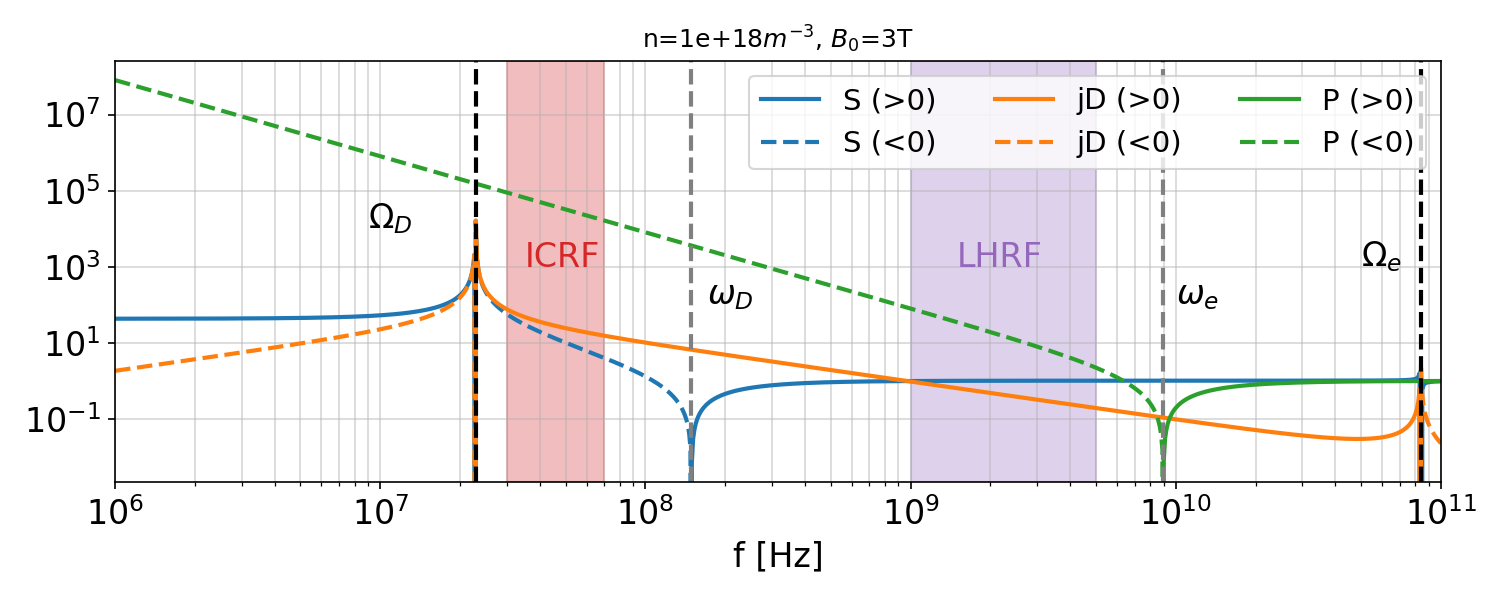
\includegraphics[width=1.0\linewidth]{figures/chap2/SDP_vs_f_nfixed_Bfixed}
	\caption{Values of the $S$, $D$, $P$ for a Deuterium plasma for density and magnetic field representative of the one we could find in front of a Tore Supra/WEST antenna. The typical Ion Cyclotron and Lower Hybrid range  of frequencies are indicated for convenience.}
	\label{fig:sdpvsfnfixedbfixed}
\end{figure*}

The form of Eq.(\ref{eq:stix_K}) is a consequence of the fact that the cold plasma is a gyrotropic media. Gyrotropic media are characterized by their invariance under any rotation about the direction of anisotropy~\sidecite{Mackay2010}, in our case the direction of the magnetic field $\Bbf_0/B_0=\mathbf{z}$. Hence, this tensor can be equivalently re-expressed into a rotation frame $(\mathbf{u}_{+}, \mathbf{u}_{-},  \mathbf{z})$, with $\mathbf{u}_{\pm}=(\mathbf{x}\pm \mathbf{y})/\sqrt{2}$:  
\begin{equation}
\Kbf(\omega)
=
\left(\begin{array}{ccc}
R & 0 & 0\\
0 & L & 0\\
0 & 0 & P
\end{array}\right)
\label{eq:stix_K_RLP}
\end{equation}
where $R$ is the \textit{right-hand} polarized component and $L$ is the \textit{left-hand} polarized component, defined as:
\marginnote{And inversely:, 
	$$
	S =  \frac{1}{2}\left(R+L\right)
	$$ 
	$$ 
	D = \frac{1}{2}\left(R-L\right)
	$$
Letters $S$, $D$, and $P$ originally come from \textit{sum}, \textit{difference} and \textit{plasma} terms \cite{stix1992}.}
\begin{subequations}
	\begin{eqnarray}
	R(\omega) 
	& = S + D = & 
	1-\sum_{s}\frac{\omega_{s}^{2}}{\omega(\omega+\Omega_{s})}
	\label{eq:stix_R}
	\\
	L(\omega)
	& = S - D = & 
	1-\sum_{s}\frac{\omega_{s}^{2}}{\omega(\omega-\Omega_{s})}
	\label{eq:stix_L}
	\end{eqnarray}
	\label{eq:stix_RL}
\end{subequations}


% ##########################################################
% ##########################################################
\subsection{Cold Plasma Dispersion Relation}
Starting from wave equation Eq.(\ref{eq:wave_equation_nxnxE}) and using that the equivalent cold plasma dielectric tensor Eq.(\ref{eq:stix_K}), one obtain:\marginnote{It is supposed that the plasma is invariant along the $\mathrm{y}$ direction, which is equivalent to say that $n_y=0$.}
\begin{equation}
\left(\begin{array}{ccc}
S - n_{z}^{2} & jD & n_{x}n_{z}\\
-jD & S - n_{x}^{2} - n_{z}^{2} & 0\\
n_{x}n_{z} & 0 & P - n_{x}^{2}
\end{array}\right)\left(\begin{array}{c}
E_{x}\\
E_{y}\\
E_{z}
\end{array}\right)=\mathbf{0}
\label{eq:relation_disp_matr_froid}
\end{equation}

The parallel direction is defined as the direction of the total confining magnetic field $\Bbf_0$. We define the \textit{parallel index} $n_\parallel$ as $n_\parallel = \mathbf{n}\cdot\Bbf_0/B_0$. We have in addition $n_{\parallel}=n_{z}$ from the frame we have defined above. The perpendicular direction is thus $n_{\perp}^{2}=n_{x}^{2}=n^{2}-n_{\parallel}^{2}$ and oriented along $\mathbf{x}$. The wavenumber spectrum in the toroidal and poloidal direction is imposed by the geometry and the RF amplitude and phase excitation of the antenna. The perpendicular index in the radial direction is then deduced from the dispersion relation, which with these notations reads to:
%\begin{marginlisting}
%Convenient \texttt{SymPy} script to obtain this result:
%\begin{lstlisting}[language=Python, basicstyle=\tiny]
%from sympy import *
%nx, ny, nz = symbols('n_x n_y n_z')
%S, D, P = symbols('S D P')
%M = Matrix([[S-nz**2, I*D, nx*nz], 
%			[-I*D, S-nx**2-nz**2, 0], 
%			[nx*nz, 0, P-nx**2]])
%M.det().factor(nx)
%\end{lstlisting}
%\end{marginlisting}

\begin{equation}
A n_{\perp}^{4} + B n_{\perp}^{2} + C = 0
\label{eq:cold_plasma_dispersion_relation_n_perp}
\end{equation}
with\marginnote[+3cm]{Where we have used $S^{2}-D^{2}=RL$.}\sidenote{NB: some signs are reversed from the solutions usually found in the literature, due to the choice of the harmonic sign $e^{j\omega t}$}:
\begin{subequations}
	\begin{eqnarray}
		A & = & S\\
		B & = & D^2 - (S - n_\parallel^2)(S + P)\\
		  & = & -RL - PS + n_{\parallel}^{2}(S+P) \nonumber \\
		C & = & P[(S - n_{\parallel}^{2})^{2} - D^2] \\
		  & = & P(n_\parallel^2 - R)(n_\parallel^2 - L) \nonumber
		\end{eqnarray}
		\label{eq:cold_plasma_dispersion_relation_n_perp_ABC}
\end{subequations}

As $S$, $D$ and $P$ do not depend on $\mathbf{n}$, Eq.(\ref{eq:cold_plasma_dispersion_relation_n_perp}) is a simple quadratic equation for $n_\perp^2$, which gives two solutions:
\begin{equation}
	n_\perp^2 
	=
	\frac{-B \pm  \sqrt{B^2 - 4AC}}{2A}
	\label{eq:nperp_solution_general}
\end{equation}
Except for some particular cases not discussed here, the discriminant $B^2 - 4AC$ is most of the time positive. This leads to two possible modes of plasma waves, called \textit{Fast} and \textit{Slow} wave modes. These names come from that the fast wave has a higher phase velocity than the slow wave. Depending on the sign of the $n_\perp^2$ solution, these waves will be either propagating ($n_\perp^2>0$) or evanescent ($n_\perp^2<0$). As seen in next sections, evanescent modes play an important role in the antenna region, in particular for coupling calculations. The antenna region is outside of the confined plasma, where the magnetic field line are open, which is called the \textit{scrape-off layer} (SOL). 


For certain values of the parameters, $n_\perp^2$ goes to zero or infinity, called \textit{cut-off} ($n_\perp^2 = 0$) or \textit{resonances} ($n_\perp^2\to\infty$) respectively \sidecite{Allis2003}. It is also possible that the two waves coalesce in a single mode, when the discriminant is zero. 
%From Eqs.(\ref{eq:nperp_solution_general}-\ref{eq:cold_plasma_dispersion_relation_n_perp_ABC}) cut-off will occur when:
%\begin{equation}
%	P = 0 \mbox{ or } R = 0 \mbox{ or } L= 0
%\end{equation}

Much of the essential physics of the wave propagation in tokamak magnetized plasma can be understood using this simplified (slab) geometry. However, so far, we have assumed that the plasma was homogenous in order to use a plane wave expansion of the electromagnetic quantities in the $(\kbf,\omega)$ domain. However, it is not the case in reality as the density and magnetic field increase as we move away from the antenna. The hypothesis that the plasma is homogeneous is similar to assuming that phenomena take place on space scale $\Delta r$ much larger than the RF wavelength. This criteria would be fulfilled if:
\begin{equation}
	\Delta r \gg \max\lambda 
	= 
	\max \frac{\lambda_0}{\sqrt{\min \varepsilon_{r}}}
	=
	\frac{\lambda_0}{\sqrt{\min\left(|S|,|D|,|P|\right)}}
\end{equation}




%which assumes that the inhomogeneity is in the $x$-direction which is also the direction of $k_\perp$. Modelling the wave in the equatorial plane of the tokamak. $k_y$ set to zero without adding anything essential to the conclusions


% ###################################################
% ###################################################
% ###################################################
\subsection{Ion Cyclotron Range of Frequencies}\label{sec:icrh}
Plasma heating of a tokamak plasma by wave coupling in the Ion Cyclotron Range of Frequencies (ICRF) requires injecting waves at a frequency $\omega$ in order to satisfy somewhere in the plasma the resonance condition\sidecite{adam1987}:
\begin{equation}
	\omega - p \Omega_i - k_\parallel v_{\parallel,i} = 0
\end{equation}
where $p$ is the cyclotron harmonic number, $\Omega_i$ the ion cyclotron angular frequency and $v_{\parallel,i}$ the parallel component of the velocity of a given species. In present tokamaks, the desired RF frequency band is around 30-70~\si{MHz}. Typical values of parameters $S$, $D$ and $P$ are illustrated in Figure~\ref{fig:icsdp}. In this range of frequency we have the ordering $\omega \ll \omega_{pe},\Omega_{ce}$ which allows to simplify a bit the previous equation. In such case, Eqs.(\ref{eq:stix_SDP}) can be further simplified for the case of a single ion species plasma to:
\marginnote{Typically, $S \ll -1$ in the plasma and change sign when crossing the so-called \textit{hybrid} resonance (where $S=0$). $D$ is mostly $\gg 1$ while $P\ll -1$. }
\begin{subequations}
	\begin{eqnarray}
		S &\approx& \frac{\omega_{i}^2}{\Omega_{i}^2 \left(1 - \omega^2/\Omega_{i}^2 \right)} \\
		D &\approx& - S \frac{\omega}{\Omega_i} \\
		P &\approx& - \frac{\omega_{e}^2}{\omega^2}  \\
		R &\approx& \frac{\omega_i^2}{\Omega_i^2 \left(1+\omega/\Omega_i\right) } \\
		L &\approx& \frac{\omega_i^2}{\Omega_i^2 \left(1-\omega/\Omega_i\right) } 
	\end{eqnarray}
\end{subequations}

\begin{figure*}[h]
	\centering
	\includegraphics[width=1.0\linewidth]{figures/chap2/IC_SDP}
	\caption{Typical values of $S$, $D$ and $P$ terms in the Ion Cyclotron Range of Frequency for the Tore Supra/WEST tokamak as a function of the electron density $n_e$ ($B_0=3\si{T}$, $f=55\si{MHz}$, $k_\parallel=9 k_0$).}
	\label{fig:icsdp}
\end{figure*}



% ###################################################
% ###################################################
\subsubsection{ICRF Dispersion Relation}
The roots of the dispersion equation Eqs.(\ref{eq:nperp_solution_general}) are approximatively\sidenote{Except close to the LH resonance} in the ICRF \sidecite{Brambilla1998, usoltceva2019}: 
\begin{subequations}
\begin{eqnarray}
n_{\perp, F}^2 &\approx& \frac{\left(R - n_\parallel^2 \right)\left(L - n_\parallel^2\right)}{S-n_\parallel^2} \\
			   &\approx& \left(S-n_\parallel^2 \right) - \frac{D^2}{S-n_\parallel^2} \nonumber \\
n_{\perp, S}^2 &\approx& \frac{P}{S}\left(S - n_\parallel^2 \right)
\label{eq:n_perp_square_approx_ICRF}		  
\end{eqnarray}
\end{subequations}
where the subscript $_F$ and $_S$ stands for \textit{Fast} and \textit{Slow} wave modes. The Figure~\ref{fig:nperpsquarevsne_ICRF} illustrates the typical range of $n_\perp^2$ values in tokamak plasma in the Ion Cyclotron Range of Frequency. 

\begin{figure*}
	\centering
	\includegraphics[width=1.0\linewidth]{figures/chap2/n_perp_square_vs_ne_ICRF}
	\caption{Perpendicular index $n_\perp^2$ from Eqs.(\ref{eq:nperp_solution_general}) (or Eqs.(\ref{eq:n_perp_square_approx_ICRF})) for Slow and Fast waves for the typical range of electron density $n_e$ found in front of tokamak ICRF antenna ($f=50\,\si{MHz}$, $B_0=3\,\si{T}$). As antennas radiate a continuous spectrum of parallel indexes $n_\parallel$, low and high values are indicated.}
	\label{fig:nperpsquarevsne_ICRF}
\end{figure*}

The Figure~\ref{fig:nperpsquarevsne_ICRF} shows that the Fast Wave mode, the one which is desired for heating the ions of the core plasma, becomes propagative for electron density beyond a \textit{cut-off} density $n_{c}$. In the ICRF, the Fast wave is evanescent up to the R-cut-off defined as: 
\begin{equation}
n_\parallel^2 = R
\end{equation}
which leads for a single ion plasma to a cut-off density $n_c$: 
\begin{equation}
	n_{e,c}
	\approx
	\frac{c^2 \varepsilon_{0} m_p}{e^2}
	\left(k_\parallel^2 - k_0^2 \right)
	\frac{\Omega_{cH}}{\omega_0}
	\left[1 + \frac{Z}{1-Z+A\omega_0/\Omega_{cH}}\right]
\end{equation}
%\begin{equation}
%n_c \approx \Omega_i^2 \frac{\left(1 + \frac{\omega}{\Omega_i}\right)}{\frac{Z^2 e^2}{\varepsilon_{0} m_i}}n_\parallel^2 
%\end{equation}
\begin{marginfigure}
	\centering
	\includegraphics[width=1.0\linewidth]{figures/chap2/core_edge_antenna}
	\caption{Illustration of the different regions in a tokamak. The core plasma is confined by following closed magnetic lines. The region defined by open field lines is the region where lie the antennas. The fast waves generated by the IC antennas are propagative only if the density is higher than a threshold, a cut-off density.}
	\label{fig:coreedgeantenna}
\end{marginfigure}
where $\Omega_{cH} = eB/m_p$, $A$ being the mass number and $Z$ the atomic number. This density depends on the RF frequency, the magnetic field and the parallel index excited by the antenna. It increases with the parallel wavenumber ($\propto k_\parallel^2$), which itself depends on the antenna phase excitation. For effective tunnelling of the Fast wave launched by the antenna, located outside the unconfined region, the plasma density in front of the antenna should be as high as possible, which highly depends on the distance between antennas and plasma. Hence, this often requires the antenna to be close as possible to the confined plasma, as illustrated in Figure~\ref{fig:coreedgeantenna}. However, this proximity has drawbacks: the heat fluxes from the plasma are impacting the antenna are higher and must be evacuated efficiently, leading to engineering issues.


% ###################################################
% ###################################################
\subsubsection{ICRF Wave Polarization}
Injecting the previous solutions into Eq.(\ref{eq:relation_disp_matr_froid}) leads to the polarization of these modes ($n_y=0$):
\begin{subequations}
	\begin{eqnarray}
		\mbox{Fast wave: } & E_z = 0 & \frac{E_x}{E_y}=\frac{j D}{S - n_\parallel^2} \\
		\mbox{Slow wave: } & E_y = 0 & \frac{E_x}{E_z}=- \frac{n_\parallel n_{\perp,S} }{S - n_\parallel^2}
	\end{eqnarray}
\end{subequations}

The key engineering issue in designing a ICRH antenna is to effectively radiate fast waves and not slow waves, as slow waves may create undesirable effects on the plasma known as \textit{RF sheaths}\sidenote{RF sheaths are briefly discussed in Section~\ref{sec:RF_sheaths}).}.

% ###################################################
% ###################################################
\subsubsection{ICRF Antennas Main Figures of Merit}
The effectiveness of Fast wave coupling is in practice measured by the maximum radiated power $P_{\mathrm{rad,max}}$ by an antenna to a given plasma and can be defined in various ways. Assuming the antenna is modelled by a lossless transmission line of characteristic impedance $Z_0$ loaded with a  resistance $R_c$, the maximum power delivered to the load would be:
\begin{equation}
P_\mathrm{rad,max} = \frac{1}{2} R_c I^2_{\mathrm{max}} = \frac{R_c}{2 Z_0^2} V_\mathrm{max}^2
\end{equation}
where $I_\mathrm{max}$ and $V_\mathrm{max}$ are the maximum peak RF current and voltage at the load. The amplitude of the maximum current on the transmission line $I_\mathrm{max}$ depends on the geometry of antenna system and of the plasma parameters. Hence, $R_c$ can be seen as a measure of the system coupling efficiency and is called the \textit{coupling} or \textit{loading} resistance. In reality however, the RF current or voltage along the strap are not constant, hence the coupling resistance can be defined using the integral over the arc length $s$ along the strap:
\begin{equation}
	R_c = \frac{2 P_{\mathrm{rad}}}{\int_s |I(s)|^2 \diff s}
\end{equation}
where $P_\mathrm{rad}$ is the time-averaged radiated power. In numerical simulation, this power can be obtained from the Poynting theorem in the $\kbf$-space as:
\begin{equation}
	P_\mathrm{rad}
	=
	\Re
	\left\{ 
	\frac{k_{0}^{2}}{4\pi^{2}}
	\iint
	\left[
	\Ebf \left(n_{y},n_{\parallel}\right)
	\times
	\Hbf^{*} \left(n_{y},n_{\parallel}\right)
	\cdot\hat{\xbf}
	\right]
	\right\} 
	\diff n_y 
	\diff n_\parallel
\end{equation}
During experiment, it can be obtained from power, voltage or current measurements, and its definition also vary from machine to machine. ICRF coupling theory is discussed in details \sidecite{messiaen1982} and compared with experiments in \sidecite{koch1988}.


The scaling of $R_c$ for an increasing electron density with a gradient length $d_c$ from the antenna to the cut-off density $n_c$,  is given by:
\begin{equation}
	R_c \propto \exp\left(- \nu \left< k_\parallel \right> d_c \right)
\end{equation}
where $\nu$ is a constant constant representing the plasma density and its gradient and $\left< k_\parallel \right>$ a characteristic factor depending on an integration over the radiated spectrum by the antenna.  On Tore Supra, this scaling has been shown to be\sidecite{clairet2004}:
\begin{equation}
R_c \propto \exp\left(- 2 \left< k_\parallel \right> d_{\mathrm{sco}} \right)
\end{equation}
where $d_{\mathrm{sco}}$ is the distance from the antenna straps to the density cut-off location. 
%KSTAR \sidecite{bae2003-1, wang2010}







% ###################################################
% ###################################################
% ###################################################
\subsection{Lower Hybrid Range of Frequencies}\label{sec:lhcd}
In the Lower Hybrid Range of Frequencies, i.e. for $\Omega_i \ll \omega \ll \Omega_e$, the $S$, $D$ and $P$ parameters can be simplified at the lead order \cite[p.222]{Brambilla1998} to (Figure~\ref{fig:lhsdp})):
\begin{subequations}
	\begin{eqnarray}
		S &\approx& 1 - \frac{\omega_i^2}{\omega^2} + \frac{\omega_e^2}{\Omega_e^2} \approx 1 \\
		D &\approx& - \frac{\omega_e^2}{\omega \Omega_e} \approx 0 \\
		P &\approx& 1 - \frac{\omega_e^2}{\omega^2} = 1 - \frac{n_e}{n_c}
	\end{eqnarray}
\end{subequations}
where $n_c$ is the cut-off density for the Slow-wave defined for $P=0$ or, more conveniently:
\begin{equation}
	n_c = \frac{m_e \varepsilon_{0}}{e^2} \omega^2 \approx  0.0124 f^2
	\label{eq:lh_cutoff_density}
\end{equation}
with $f$ specified in $\si{GHz}$ and $n_c$ given in $10^{18}\si{m^{-3}}$ 
\begin{figure*}[h]
	\centering
	\includegraphics[width=1.0\linewidth]{figures/chap2/LH_SDP}
	\caption{Values of $S$, $D$ and $P$ terms in the Lower Hybrid Range of Frequency. ($f=3.7\,\si{GHz}$,$B_0=3\,\si{T}$).}
	\label{fig:lhsdp}
\end{figure*}


% ###################################################
% ###################################################
\subsubsection{LHRF Dispersion Relation}
In the LHRF, the solution of the dispersion relation reads:
\begin{subequations}
	\begin{eqnarray}
		n_{\perp,F}^2 &\approx& S - n_\parallel^2  \approx 1 - n_\parallel^2 \\
		\label{eq:n_perp_square_FW_LHRF}
		n_{\perp,S}^2 &\approx& \frac{P}{S} \left(S - n_\parallel^2\right) \approx P(1- n_\parallel^2)
		\label{eq:n_perp_square_SW_LHRF}
	\end{eqnarray}
	\label{eq:n_perp_square_LHRF}
\end{subequations}

\begin{figure*}[h]
	\centering
	\includegraphics[width=1.0\linewidth]{figures/chap2/n_perp_square_vs_ne_LHRF}
	\caption{Perpendicular index $n_\perp^2$ from Eqs.(\ref{eq:nperp_solution_general})   for the typical range of electron density $n_e$ found in front of tokamak LHRF antenna ($f=3.7\,\si{GHz}$, $B_0=3\,\si{T}$).}
	\label{fig:nperpsquarevsne_LHRF}
\end{figure*}

% ###################################################
% ###################################################
%\subsubsection{Resonance Cone}
%Bellan and Porkolab PRL 34, 124, 1975.

% ###################################################
% ###################################################
\subsubsection{LHRF Wave Polarization}
Similarly, the electric field polarisation in the LHRF gets ($n_y=0$):
\begin{subequations}
	\begin{eqnarray}
	\mbox{Fast wave: } & E_z = 0 & \frac{E_x}{E_y}= \frac{j D}{S - n_\parallel^2} \\
	\mbox{Slow wave: } & E_y = 0 & \frac{E_x}{E_z}=- \frac{n_\parallel n_{\perp,S} }{S - n_\parallel^2}
	\end{eqnarray}
\end{subequations}

% ###################################################
% ###################################################
\subsubsection{Wave propagation conditions}
In order for the RF power to reach the plasma core, the excited waves by a LHCD launcher must satisfy different criteria: 

\begin{itemize}
	\item  A \emph{cut-off condition}: the electron density in front of the launcher must be close or higher than the slow-wave electron \emph{cut-off density}, given by Eq.(\ref{eq:lh_cutoff_density}), that increases as the square of the source frequency. 
	\item A propagation condition: in order for the Slow and Fast waves in the LHRF to propagate into the magnetized plasma, from Eqs.(\ref{eq:n_perp_square_LHRF}) excited waves must have an absolute value of the parallel index greater than one, i.e. $|n_{\parallel}|>1$ 
	\item An accessibility condition: in order for the Slow waves accessing the plasma core to not be mode-converted into Fast waves, a minimum value of $n_{\parallel}$ for a given plasma density and magnetic field is requested\sidecite{golant1972}:
	\begin{equation}
	|n_{\parallel} |>| n_{\parallel \mathrm{access}} | 
	\approx 
	\sqrt{1 
		- \frac{\omega_{pi}^2}{\omega^2} 
		+ \frac{\omega_{pe}^2}{\omega_{ce}^2}}
	+ \frac{\omega_{pe} }{| \omega_{ce} |}
	\label{eq:accessibilit_condition_LH}
	\end{equation}
\end{itemize}

When the accessibility condition is satisfied, the Slow and Fast branches of the dispersion relation are separated and the LH waves can reach the core plasma. Inversely, for a given $n_{\parallel}$, the previous condition leads to an upper limit for the density (inside the plasma), above which the wave can’t propagate.

% ###################################################
% ###################################################
\subsubsection{LHRF Antennas Main Figures of Merit}
There are three important figures of merit to measure the efficiency and
performance of a LH launcher. The first one is the $\mathbf{k}$-space radiated power spectrum density $ p(n_y, n_\parallel)$, defined as the $k$-space Poynting vector\marginnote{Integrating the power spectrum density over the entire $n$-space gives the transmitted power to the plasma.}:
\begin{equation} 
 p
\left(n_{y},n_{\parallel}\right)
=\Re\left\{ \frac{k_{0}^{2}}{4\pi^{2}}
\left[\tilde{\mathbf{E}}
\left(n_{y},n_{\parallel}\right)
\times
\tilde{\mathbf{H}}^{*}\left(n_{y},n_{\parallel}\right)
\cdot\hat{\xbf}
\right]
\right\} 
\end{equation}
Since it is often assumed that the plasma is infinite in the $y$ direction (slab model), the main acceptation of the power spectrum density is $ p(n_\parallel)$, which corresponds to integrate the contribution of all the $n_{y}$ for a given $n_{\parallel}$:
\begin{equation}
 p\left(n_{\parallel}\right)=\int_{-\infty}^{+\infty}\!  p\left(n_{y},n_{\parallel}\right)\, \diff n_y
\end{equation}
This quantity represents the amount of power excited by the launcher for each parallel index $n_\parallel$. % The relation between this power spectrum and the array excitation is related to the Fourier transform of the electromagnetic field at the plasma-antenna interface.

The second one is the ratio of the reflected power (at the mouth or at the end of the launcher) to the input power, named the reflection coefficient $|\Gamma|^2 $ and often expressed in percent:
\begin{equation}
	|\Gamma|^2 = P_r/P_i
\end{equation} 

The third one is the directivity of the launcher, which is the fraction of the power spectrum over its total power content. It can be viewed as the fraction of the power that goes toward one toroidal direction over the total coupled power. One can define the directivity as:
\begin{equation}
\mathrm{Dir} = \frac{\int_{n_\parallel > 0}   p(n_\parallel) \diff n_\parallel}{\int  p(n_\parallel) \diff n_\parallel} 
\end{equation}

Since the wave field at the launcher aperture (and thus the launcher spectrum) depends on both the antenna and the plasma, numerical coupling codes are required to make a self-consistent numerical evaluation of the coupling. Different types of launchers have been developped to balance the sometimes conflicting requirements of experimental flexibility, reduced complexity and thermal constraints. These antennas are discussed in Section~\ref{sec:LHCD_antennas_general}.


%The RF power is coupled by the launcher to the plasma, which means that the electromagnetic waves in the launcher’s waveguides are converted to (mainly) slow waves in the plasma. In the LH range of frequencies (~2 to 8 GHz), the wavelength of the RF waves in the plasma is well below the typical beam size, which itself is smaller than the equilibrium non-uniformity scale. It this situation, the evolution of the waves in the plasma can be described by the \emph{ray-tracing} formalism. Since the evolution of the electron population can be described with Fokker-Planck calculation, the combination of the both tools is standard for modelling LHCD experiments\sidecite{bonoli1982, peysson2012}.
%
%As said before, the LHCD launcher is a phased array of waveguide which excites a slow plasma wave. The following calculations taken from current drive theory illustrate the basic requirements of the LHCD launcher in order to optimize the current drive efficiency. 
%
%In the plasma, the incremental current $\Delta j$ carried by an electron of electrical charge $q=-e$ and accelerated from a parallel velocity $v_\parallel$ to $v_\parallel + \Delta v_\parallel$ is:
%$$\Delta j = q \Delta v_{\parallel}$$
%
%The incremental increase of kinetic energy is:
%$$\Delta E = m v_{\parallel} \Delta v_{\parallel}$$
%
%Eliminating $\Delta v_{\parallel}$ leads to an incremental current: 
%$$\Delta j = \Delta E \; q/(m v_{\parallel})$$ 
%
%Let $\nu_\mathrm{coll}$ be the Coulomb collisional frequency. At first order \footnote{Rigourously, the mathematical tool for a complete description of multiple scattering processes in the velocity-space is the Boltzman equation. The collision term modelling the multiple particles Coulomb collisions in this equation can be modelled by a collision term of the Fokker-Planck type.} the incremental energy input $\Delta E$ persists for a time $1/\nu_\mathrm{coll}$. The associated (steady-state) RF input power $\Delta P$ required is thus: 
%$$\Delta P = \nu_\mathrm{coll} \Delta E$$ 
%
%From the two previous equations, the ratio of the incremental current to the RF input power is:
%$$\Delta j/ \Delta P = q / (m \nu_\mathrm{coll} v_{\parallel})$$
%
%This suggests that more current can be driven with low parallel velocity electrons. However, fast electrons collide less often than slower, as the Coulomb collision cross section falls off with increasing relative velocity as $\nu_\mathrm{coll} \propto n_e/v_{\parallel}^3$ (for parallel velocity larger than the thermal velocity). It follows that the previous ratio is proportional to: 
%
%$$\Delta j/ \Delta P \propto (v_{\parallel}^2 q) / (m n_e)$$
%
%this means that high current drive efficiency can be reached from fast electrons. Thus, it is actually more effective to push fast electrons than slower. Even if it may be energetically more expensive to accelerate fast electrons, this energy deposition need occurs less often because current last longer when carried by relatively less collisional electrons \sidecite{fisch1987}. 
%
%For the purpose of current drive with LH waves, the Landau damping is the dominant absorption mechanism. Landau damping is a collision-less damping process in which particles exchange energy with waves travelling with the nearly same phase velocity parallel to the magnetic field, that is, for particle parallel velocity $v_{\parallel}$ satisfying resonant condition:
%
%$$\omega – k_{\parallel} v_{\parallel} = 0 $$ 
%
%where $k_{\parallel}=k_0 n_{\parallel}$ is the parallel wavenumber of the wave, $n_{\parallel}$ the parallel index of refraction and $k_0= \omega/c$ the wavenumber in vacuum. From the previous relation one deduces that the LHCD launcher must excite waves satisfying the resonant condition $v_{\parallel}=c/n_{\parallel}$. As for the slow wave to be able to penetrate into the plasma the parallel index must be greater than one and also greater to $|n_{\parallel \mathrm{access}}|$, typical LHCD launchers in current tokamaks excite a main parallel index between $n_{\parallel 0}$=1.5 to 3.0. 
%
%However, in many past and present LHCD experiments, the resonant velocity $v_{\parallel 0}=c/n_{\parallel 0}$ corresponds to supra thermal region where the number of electrons should be in principle too small for any significant wave damping to take place and to account for the observed current drive. Indeed, strong wave damping on a Maxwellian distribution with temperature $T$ requires the wave damping to be no larger than four times the thermal velocity $v_T=\sqrt{k T/m}$. This paradox is commonly referred to as the \emph{spectral gap} problem and is an active area of research. Various explanations are proposed to explain this spectral gap, among these the toroidal effects on the wave propagation that can cause sufficient up-shift (increase of the parallel wavenumber) in the parallel refraction index $n_{\parallel}$ to “fill” the spectral gap, non-linear interactions such as \textit{parametric decay instabilities} (PDI), diffraction effects or power density spectrum fluctuations. 



\clearpage
% ###################################################
% ###################################################
\section{The ALOHA code}\label{sec:ALOHA}
\marginnote{Parts of this section are taken from paper \citeauthyear{hillairet2010}.}
% ###################################################
\subsection{Context of this work}
The theory of the coupling between LHRF antennas and the plasma has been developed in \sidecite[-0.5cm]{brambilla1976-1,brambilla1979} for 2D waveguides (parallel plates infinite the poloidal direction) and refined after for rectangular waveguides in \sidecite{bers1983}. In 2007, best known linear coupling codes used to design present operating antennas are Slow Wave ANtenna (SWAN) \sidecite{litaudon1990, moreau1984} or GRILL3D \sidecite[+1cm]{irzak1995}. In these codes, the toroidal lines of waveguides are assumed to be infinite in the poloidal direction and are described using a modal expansion. The modal description of the field makes possible to simulate large antennas with a moderate computing cost but the code cannot handle realistic geometry.

In order to improve the antenna-plasma coupling description of SWAN code while keeping its low computational cost, a code named Advanced LOwer Hybrid Antenna (ALOHA) has been developed\sidenote{The code has been initially written by S.Berio and Ph.Bibet in 1994 \cite{berio1996}, then improved later by Damien Voyer in 2006. Since 2008, I continued to develop the code, completely rewritten since in modern Fortran with a Matlab front-end. The code development was first versioned on CEA internal servers since Nov.2009 before being \href{https://github.com/jhillairet/ALOHA}{open-sourced in on github} since Sept.2015. ALOHA has been used by different user in fusion laboratory worldwide: MIT/PSFC, ASIPP, NFRI, IPR, IPP/Prague, etc. Since 2008, ALOHA has been cited in more than 130 references.}. In ALOHA, LH antennas may be modelled by any RF full-wave commercial software or home-made code\footnote{For optimization process, a plug-in named HAMAC (Hybrid Antenna Modelling for the ALOHA Code) has been developed in the frame of the master training of Melanie Preynas in 2009 and Michal Kazda in 2010.}. The plasma coupling is calculated from a fast classical 1D modelling that describes the effect of the slow wave only\cite{brambilla1976-1} or from a more advanced 2D modelling that implies the contribution of both fast and slow waves\cite{brambilla1979, bers1983, irzak1995}.
These calculations are based on the linear cold plasma theory and non-linear effects, such as thermal effects ("warm" dielectric tensor) and ponderomotive force have not been taken into account in the present analysis. However, some specific developments have been brought in one hand, to describe a more realistic electron density profiles taking into account the close environment of LH antennas and in the other hand, to avoid computational difficulties when the antenna is large. These assumptions let ALOHA to solve a case in a couple of seconds up to 2 hours on a 2008 desktop computer, depending on the number of waveguides of the antenna and the plasma model chosen. By comparison, a boundary element code such as the Torino Politecnico Lower Hybrid Antenna (TOPLHA) code\sidecite{milanesio2011}, required at that time high-end or super-computers to be solved. At the same time, finite element software such as COMSOL just began to be able to treat materials with generic temporally-dispersive dielectric tensors. Such approach leaves absolute freedom in the description of the antenna geometry and of the plasma within the collisional cold plasma approximation but required high computation time or resources \sidecite{meneghini2009-1, shiraiwa2011-1}. Nowadays, the Finite-Element Method can be used in more daily basis for LHCD coupling as discussed in Section~\ref{sec:LHCD_FW_antena_coupling}. However, it is still incompatible with intensive use, for example in daily experiments when one has to evaluate the effect of modules tripping on the radiated spectrum or during antenna design stage, where many calculations may be expected. In order to interpret and improve present day experiments and to design future antennas, an advanced but fast and convenient modelling tools is still convenient.

The next section recalls the key elements of the linear coupling theory. ALOHA specificities are detailed, such as the use of generalized scattering matrix, the 2D grill modelling and the two electron density gradients profile. Section~\ref{sec:ALOHA_TS} is devoted to experimental comparisons and simulation benchmarks on Tore Supra antennas. 


\subsection{Main assumptions}\label{sec:Theory}

\subsubsection{Network description}\label{sec:network_description}

The LHCD antennas of past or present experiments (JET, Alcator C-Mod, FTU, EAST, KSTAR, Tore Supra/WEST, etc.) are designed to launch an asymmetric parallel wavenumber spectrum where most of the power is generated at a low parallel refractive index $\left|n_{\parallel}\right|\approx2$. This is usually achieved by phasing the forward waves in waveguides that are stacked along the static magnetic field. This phasing can be obtained externally in the transmission line feeding of the antenna \sidecite[-2cm]{bernabei2003, bae2003, park2010} or directly inside the antenna when E-plane power dividers -- usually called "multijunction" \sidecite{moreau1984} -- are associated with built-in phase shifters \sidecite[+0.5cm]{ekedahl2009-1, bo-jiang2006, zhao2010}.

Here, the term "module" refers to the unit of the antenna composed of one "input" waveguide fed by the power source and one or several "output" waveguides facing the plasma, and the "grill" refers to the plane containing all the open ended waveguides of the antenna. A complete LH antenna can be made of many different modules, stacked in the toroidal or poloidal directions. A simple example is depicted in Figure~\ref{fig:geometry_antenna}.

In the ALOHA code, the plasma coupling of a LH grill antenna is split into two parts: the modeling of the modules and the modeling of the grill in front of the plasma. 

Firstly, the electromagnetic characterization of a module is obtained using some RF software or code, which results in the calculation of the scattering matrix of a module $\mathbb{S}_{\mbox{module}}$ in which only the propagating modes are taken into account. This matrix quantifies the coupling between all inputs and outputs of the RF structure \cite{kurokawa1965}. 

Secondly, the coupling to the plasma of all the output waveguides that compose the grill is considered. At this stage, evanescent modes excited at the end of the waveguides are also taken in account. Thus, the grill is characterized by a $N$-port network where $N=N_{\mbox{wg}}\times N_{\mbox{modes}}$ is the number of ports, $N_{\mbox{wg}}$ the total number of output waveguides and $N_{\mbox{modes}}$ the number of electromagnetic modes in each waveguide. A scattering matrix $\mathbb{S}_{\mbox{grill/plasma}}$ of dimensions $N\times N$ is then derived using the approach detailed in Section~\ref{sec:grill_modeling}: this matrix quantifies the coupling between the different ports. In such a modeling, each mode is associated to a port \cite{Harrington2001}; a port can coincide either with the principal mode that propagates inside an output waveguide or with a higher order mode excited at the end of an output waveguide. 

Finally, following the well known network approach, both modellings are combined: the ports in the scattering matrices $\mathbb{S}_{\mbox{module}}$ and $\mathbb{S}_{\mbox{grill/plasma}}$ that correspond to the same mode in a waveguide are identified and the global response of the antenna can then be extracted and directly compared to experimental data.

For a better understanding, let us consider the example of the antenna shown in Figure~\ref{fig:geometry_antenna}. It is composed of one toroidal line of waveguides shared into two modules. Each module is a multijunction in which a large input feeding waveguide is split into four smaller output waveguides; the output waveguides are said to be active waveguides since they are connected to the input waveguide inside the module. The modules are separated by a short circuited waveguide; this waveguide is isolated and consequently is said to be passive. Moreover, there is also one passive waveguide on each side of the antenna. Each module is characterized by a scattering matrix $\mathbb{S}_{\mbox{module1}}$ and $\mathbb{S}_{\mbox{module2}}$.

%
\begin{figure}[h]
	\centering{}\includegraphics[width=0.9\textwidth]{figures/chap2/ALOHA/figure1} 
	\caption{A typical LH (multijunction) antenna structure. In this example, the
		antenna is made of two multijunction modules stacked in the toroidal
		($z$) direction. One passive waveguide is inserted between both modules
		and on each side of the antenna.\label{fig:geometry_antenna} }
	
\end{figure}


Suppose that, in front of the plasma, two modes are excited inside the output waveguides: the principal mode $\TE_{10}$ and the evanescent mode $\TM_{11}$. The network modeling of this problem is given in figure \ref{fig:network_representation}. In that representation, a port in a N-port network is described by a terminal. Thus, each of both modules is characterized by a 5-port network (1\,input waveguide $\times$ 1\,mode + 4\,active waveguides $\times$ 1\,mode) and the coupling of the grill with the plasma is modeled by a 22-port network (\textit{\emph{8\,active waveguides $\times$ 2\,modes + 		3\,passive waveguides $\times$ 2\,modes}}). The terminals in the 22-port network that coincide with the principal mode of the active waveguides in the modules are connected to the corresponding terminals in the 5-port network. The terminals in the 22-port network that coincide with the principal mode of the passive waveguides are shunt on a piece of transmission line ended by a short-circuit to model the reflection of the wave. The terminals in the 22-port network that coincide with the evanescent modes are shunt on the imaginary mode impedance of the output waveguide, which is equivalent to consider that those modes carry reactive energy in a waveguide of infinite length. Finally, the antenna reduces to a 2-port network in which the ports correspond to the input feeding waveguide of both modules and the global scattering matrix of the antenna is a $2\times2$ matrix $\left(\mathbb{S}_{\mbox{access}}\right)$. This formalism allows the code to fully take into account the coupling of the modes in the waveguides.

%
\begin{figure}[h]
	\centering{}\includegraphics[width=0.7\textwidth]{figures/chap2/ALOHA/figure2} \caption{Illustration of the modeling of the antenna described in figure \ref{fig:geometry_antenna}
		using the N-port concept.\label{fig:network_representation} }
	
\end{figure}



\subsubsection{Module modelling}\label{sub:module_modeling}

Lower Hybrid experiments show that the coupling efficiency not only depends on the plasma configuration but also on the antenna structure. Antennas are often designed in order to minimize the reflected power from the plasma to the RF sources, thus limiting the need of complex and expensive klystron protection systems. Multijunction concept is frequently used in tokamaks in order to create large waveguide arrays. The necessary phase shifts between adjacent waveguides used to launch non-symmetrical parallel wavenumber spectrum is usually obtained in the design by adjusting the relative guide heights \sidecite{litaudon1992}. These built-in phase shifters create multiple passages of the waves through the structure, which lead to a reduction of the reflected power to the RF sources as well as an increase of the electric field strength or an increase of secondary peaks in the radiated power spectrum. Thus, the RF design of such antennas is less straight-forward than simple open-ended waveguides and an accurate RF characterization is required to analyze the experimental data.

The coupling efficiency requires the measurement of the forward and reflected electric fields in all waveguides which in principle can be done but requires the installation under vacuum of a very large number of probes\sidecite{jacquet1997, meneghini2010}. For an easier maintenance of the RF system, the use of a single bi-directional coupler at the module input in the pressurized transmission line is usually preferred. With this scheme, the electric field map at the plasma-antenna interface, needed to compute the launched parallel index $n_{\parallel}$, is only accessible by computation. In order to directly compare theoretical coupling predictions to experimental RF measurements, the RF description of each module have to be considered incorporating all the RF components in line from the plasma up to the RF probes location. Thus, the realistic wave propagation inside each module, through multijunctions and power splitters (such as hybrid junctions, magic tees or mode converters) has to be taken into account. 

Commercial RF softwares, for example ANSYS HFSS, CST Studio or COMSOL, are convenient tools to design and optimize such components. In ALOHA, the scattering matrix calculated by these codes that describe the modules of the antenna can be directly used as input. Once the antenna's module scattering matrices calculated ($\mathbb{S}_{\mbox{module}}$), they are used as input for ALOHA to simulate the coupling between the modules and the plasma, as explained in the next sections.


\subsubsection{Grill-plasma modelling}\label{sec:grill_modeling}

\paragraph{Plasma description}\label{sec:dielectric_tensor}

Lets consider the geometry shown in Figure~\ref{fig:geometry_antenna}. The static magnetic field $\mathbf{B}_{0}$ is assumed to be in the $z$ direction and vary as well as the plasma density in $x$ direction. This hypothesis is specifically valid for large tokamak such as ITER or tokamak with large aspect ratio in which the angle between the magnetic field and the narrow waveguide is small. The interface between waveguides and plasma is set at $x=0$. The plasma is considered homogeneous
in $y$ and $z$ directions. The electromagnetic field scattered by the antenna is supposed to be dissipated far away from the coupling region so that the coupling problem is treated as a problem of radiation in a semi-infinite medium independently of the absorption in the core plasma. In such a modelling, the propagation into the plasma core is not calculated, meaning that effects such as mode conversion are not taken into account. 

From Maxwell's equations, we recall that the electromagnetic field in a cold plasma in the absence of source satisfies the vector wave equation:
\begin{equation}
\left(\nabla\times\nabla\times-k_{0}^{2}\mathbf{K}\cdot\right)\left|\begin{array}{c}
\mathbf{E}(\mathbf{r})\\
\mathbf{H}(\mathbf{r})\end{array}\right.=0
\end{equation}

where $\mathbf{E}$ and $\mathbf{H}$ are the electric and magnetic fields, $\mathbf{r}=x\mbox{\ensuremath{\hat{\mathbf{x}}}}+y\hat{\mathbf{y}}+z\hat{\mathbf{z}}$ is the space vector coordinates and $k_{0}=\frac{\omega}{c}$ the free-space wavenumber. In the vicinity of the grill, the plasma is described by its (normalized) cold dielectric tensor $\mathbb{K}$ Eq.(\ref{eq:stix_K}) which is recalled here: 
\begin{equation}
	\mathbf{K}(x,\omega)=\left[\begin{array}{ccc}
	S & jD & 0\\
	-jD & S & 0\\
	0 & 0 & P\end{array}\right]
	\label{eq:dielectric_tensor}
\end{equation}
where parameters $S$, $D$ and $P$ are defined by Eq.(\ref{eq:stix_SDP}) and depend on radial position $x$ and wave frequency.

%\begin{eqnarray}
%S(x,\omega) & = & 1-\sum_{s}\frac{\omega_{p,s}^{2}}{\omega^{2}-\Omega_{c,s}^{2}}\label{eq:stix_sum}\\
%D(x,\omega) & = & \sum_{s}\frac{\Omega_{ci}}{\omega}\frac{\omega_{p,s}^{2}}{\omega^{2}-\Omega_{c,s}^{2}}\label{eq:stix_difference}\\
%P(x,\omega) & = & 1-\sum_{s}\frac{\omega_{p,s}^{2}}{\omega^{2}}\label{eq:stix_plasma}
%\end{eqnarray}
%where $\omega$, $\Omega_{c,s}$ and $\omega_{p,s}$ are respectively the RF source, the cyclotron and the plasma angular frequencies of the species $s$.

% ####################################################################
\paragraph{Grill description}
The transverse (perpendicular to the $x$ direction) electromagnetic field $\mathbf{E}_{t,\mbox{grill}}$, $\mathbf{H}_{t,\mbox{grill}}$ at the end of the output waveguides, i.e. in the $x=0$ grill plane, can be expanded as a series of excited modes in similar way than Eq.(\ref{eq:voltage_current_lossy_line}) from Chap.\ref{chap:RF_fundamentals}:
\begin{eqnarray}
\mathbf{E}_{t,\mbox{grill}}(x=0,y,z) & = & \sum_{n=1}^{N}\sqrt{Z_{n}}\left(a_{n}+b_{n}\right)\mathbf{e}_{t,n}(y,z)\\
\mathbf{H}_{t,\mbox{grill}}(x=0,y,z) & = & \sum_{n=1}^{N}\frac{1}{\sqrt{Z_{n}}}\left(a_{n}-b_{n}\right)\mathbf{h}_{t,n}(y,z)
\end{eqnarray}
where $\mathbf{e}_{t,n},\,\mathbf{h}_{t,n}$ are the TE or TM modal functions (explicitly given in reference.\,\cite{Harrington2001}) associated to the port $n$ and $Z_{n}$ the impedance of the port $n$ for the current mode. The coefficients $a_{n}$ and $b_{n}$ are the incident and reflected power waves associated to the port $n$. We recall that $N=N_{\mbox{wg}}\times N_{\mbox{modes}}$ is the total number of ports, $N_{\mbox{wg}}$ being the total number of waveguides and $N_{\mbox{modes}}$ the number of modes in each waveguide. Since the analytical expression of the modes function $\mathbf{e}_{t,n},\,\mathbf{h}_{t,n}$ are known, the transverse fields can be analytically expressed in the spectral domain by Fourier transform:
\begin{eqnarray}
\tilde{\mathbf{E}}_{t,\mbox{grill}}\left(n_{y},n_{z}\right) & = & \sum_{n=1}^{N}\sqrt{Z_{n}}\left(a_{n}+b_{n}\right)\tilde{\mathbf{e}}_{t,n}\left(n_{y},n_{z}\right)\label{eq:E_grill_spectral}\\
\tilde{\mathbf{H}}_{t,\mbox{grill}}\left(n_{y},n_{z}\right) & = & \sum_{n=1}^{N}\frac{1}{\sqrt{Z_{n}}}\left(a_{n}-b_{n}\right)\tilde{\mathbf{h}}_{t,n}\left(n_{y},n_{z}\right)\label{eq:H_grill_spectral}\end{eqnarray}
where $\tilde{\mathbf{e}}_{t,n}$ and $\tilde{\mathbf{h}}_{t,n}$ are the Fourier transform of the modal functions $\mathbf{e}_{t,n},\,\mathbf{h}_{t,n}$ and $n_{y}=k_{y}/k_{0}$ and $n_{z}=k_{z}/k_{0}$ are the refractive indexes in $y$ and $z$ directions respectively. These latter expressions will be used for the coupling calculation in the next section.


\paragraph{Coupling from grill to plasma}

Following the classical linear-coupling regime \cite{brambilla1979,bers1983}, the characterization of the plasma medium can be reduced to a spectral surface admittance $\mathbb{Y}_{S}$ defined on the plane that separates the grill from the plasma region:
\begin{equation}
\tilde{\mathbf{H}}_{t,\mbox{plasma}}\left(n_{y},n_{z}\right)=Y_{0}\mathbb{Y}_{S}\left(n_{y},n_{z}\right)\tilde{\mathbf{E}}_{t,\mbox{plasma}}\left(n_{y},n_{z}\right)\label{eq:surface_admittance}
\end{equation}

where $\tilde{\mathbf{H}}_{t,\mbox{plasma}}\left(n_{y},n_{z}\right)$ and $\tilde{\mathbf{E}}_{t,\mbox{plasma}}\left(n_{y},n_{z}\right)$ are the Fourier transforms of the transverse magnetic $\mathbf{H}_{t,\mbox{plasma}}(x=0,y,z)$ and electric fields $\mathbf{E}_{t,\mbox{plasma}}(x=0,y,z)$. $Y_{0}$ is the vacuum admittance. The plasma surface admittance $\mathbb{Y}_{s}$, which is discussed in Sec.\ref{sec:surface_admittance}, is generally
a $2\times2$ complex matrix.

The waveguides of the grill are supposed to be opened through a perfect metallic surface of infinite extent. Due to the continuity of the transverse electric field in the waveguide openings and no tangent electric field on the perfect metallic surface, the transverse magnetic field $\tilde{\mathbf{H}}_{t,\mbox{plasma}}$ can be expressed using the surface admittance $\mathbb{Y}_{s}$ defined in (\ref{eq:surface_admittance}) and the expansion of the electric field $\tilde{\mathbf{E}}_{t,\mbox{grill}}$ given in (\ref{eq:E_grill_spectral}). Thus, 
\begin{equation}
\tilde{\mathbf{H}}_{t,\mbox{plasma}}\mbox{\ensuremath{\left(n_{y},n_{z}\right)}}=\sum_{n=1}^{N}\sqrt{Z_{n}}\left(a_{n}+b_{n}\right)Y_{0}\mathbb{Y}_{s}\left(n_{y},n_{z}\right)\tilde{\mathbf{e}}_{t,n}\left(n_{y},n_{z}\right)\label{eq:H_plasma_spectral}
\end{equation}

Let $\tilde{\mathbf{H}}_{t,\mbox{metal}}\left(n_{y},n_{z}\right)$ be the transverse magnetic field related to the current induced on the perfect metallic surface of infinite extent. Due to the continuity between transverse magnetic field in the waveguide openings, one finds from the expansion of the magnetic field in the grill (\ref{eq:H_grill_spectral}) and in the plasma (\ref{eq:H_plasma_spectral}) the following equality:
\begin{eqnarray}
\sum_{n=1}^{N}\frac{1}{\sqrt{Z_{n}}}\left(a_{n} - b_{n}\right)\tilde{\mathbf{h}}_{t,n}\left(n_{y},n_{z}\right) & + & \tilde{\mathbf{H}}_{t,\mbox{metal}}\left(n_{y},n_{z}\right)=\label{eq:H_continuity_spectral}\\
&  & \sum_{n=1}^{N}\sqrt{Z_{n}}\left(a_{n}+b_{n}\right)Y_{0}\mathbb{Y}_{s}\left(n_{y},n_{z}\right)\tilde{\mathbf{e}}_{t,n}\left(n_{y},n_{z}\right)\nonumber 
\end{eqnarray}

The mode matching method is then applied \cite{berio1996}: a linear system is obtained by dot product multiplying both sides of (\ref{eq:H_continuity_spectral}) with $\tilde{\mathbf{h}}_{t,m}^{*}\left(n_{y},n_{z}\right)$ for $m=1,\ldots,N$ and integrating over the spectral domain $\left\{ n_{y},n_{z}\right\} $ of infinite extent. Moreover, by multiplying both sides by $k_{0}^{2}/4\pi^{2}$, the left hand side of the equation can be transposed in the spatial domain $\left\{ y,z\right\} $ thanks to Parseval's theorem:
\begin{eqnarray}
\sum_{n=1}^{N}\frac{1}{\sqrt{Z_{n}}}\left(a_{n}-b_{n}\right)\left[\int\int_{-\infty}^{+\infty}\!\mathbf{h}_{t,m}^{*}\left(y,z\right)\cdot\mathbf{h}_{t,n}\left(y,z\right)\, dy\, dz\right.\\
\left.+\int\int_{-\infty}^{+\infty}\!\mathbf{h}_{t,m}^{*}\left(y,z\right)\cdot\mathbf{H}_{t,\mbox{metal}}\left(y,z\right)\, dy\, dz\right]=\nonumber \\
\sum_{n=1}^{N}\sqrt{Z_{n}}\left(a_{n}+b_{n}\right)C_{mn}\nonumber 
\end{eqnarray}
where the coupling admittance term $C_{mn}$ is given by:
\begin{equation}
C_{mn}=Y_{0}\frac{k_{0}^{2}}{4\pi^{2}}\int\int_{-\infty}^{+\infty}\tilde{\mathbf{h}}_{t,m}^{*}\left(n_{y},n_{z}\right)\mathbb{Y}_{s}\left(n_{y},n_{z}\right)\tilde{\mathbf{e}}_{t,n}\left(n_{y},n_{z}\right)\, dn_{y}\, dn_{z}\label{eq:coupling_admittance}
\end{equation}
Since the modal function $\mathbf{h}_{t,m}$ is zero on a perfect metallic plane, the term involving $\mathbf{H}_{t,\mbox{metal}}$ cancels. The orthonormal properties of the modal eigenfunctions\cite{Collin1990,Harrington2001}
leads to:
\begin{equation}
\frac{1}{\sqrt{Z_{m}}}\left(a_{m}-b_{m}\right)=\sum_{n=1}^{N}\sqrt{Z_{n}}\left(a_{n}+b_{n}\right)C_{mn}\qquad\forall\, m=1,\,\ldots,\, N\label{eq:linear_system}
\end{equation}
The linear system of equation.(\ref{eq:linear_system}) can be rewritten
using a matrix formalism:
\begin{equation}
\sqrt{\mathbb{Z}}^{-1}\left(\mathbf{a}-\mathbf{b}\right)=\mathbb{C}\sqrt{\mathbb{Z}}\left(\mathbf{a}+\mathbf{b}\right)\label{eq:linear_system_matrix}
\end{equation}
where $\sqrt{\mathbb{Z}}$ is diagonal matrix with $\left[\sqrt{\mathbb{Z}}\right]_{ii}=\sqrt{Z_{i}}$ and $\mathbb{C}$ is the coupling admittance matrix with $\left[\mathbb{C}\right]_{ij}=C_{ij}$. $\mathbf{a}$ and $\mathbf{b}$ are respectively the incident and reflected waves vectors associated to the port $i$, such as $\left[\mathbf{a}\right]_{i}=a_{i}$ and $\left[\mathbf{b}\right]_{i}=b_{i}$. The scattering matrix $\mathbb{S}_{\mbox{grill/plasma}}$ discussed in Section~\ref{sec:network_description} is defined by

\begin{equation}
\mathbf{b}=\mathbb{S}_{\mbox{grill/plasma}}\mathbf{a}\label{eq:Sgrillplasma_def}
\end{equation}
Finally, using (\ref{eq:linear_system_matrix}), one finds:
\begin{equation}
\mathbb{S}_{\mbox{grill/plasma}}=\left(\mathbb{I}+\sqrt{\mathbb{Z}}\mathbb{C}\sqrt{\mathbb{Z}}\right)^{-1}\left(\mathbb{I}-\sqrt{\mathbb{Z}}\mathbb{C}\sqrt{\mathbb{Z}}\right)
\end{equation}
where $\mathbb{I}$ is the unit matrix.

\subsection{Antenna power spectrum}
An important feature of LH antennas is the radiated power spectral density $p$ that can be computed from the Poynting vector: 
\begin{equation} 
 p
\left(n_{y},n_{z}\right)
=\Re\left\{ \frac{k_{0}^{2}}{4\pi^{2}}\left[\tilde{\mathbf{E}}\left(n_{y},n_{z}\right)\times\tilde{\mathbf{H}}^{*}\left(n_{y},n_{z}\right)\cdot\widehat{x}\right]\right\} 
\label{eq:power_spectrum_2D}
\end{equation}
According to previous equations, this power density can be evaluated once the power waves $\mathbf{a},\mathbf{b}$ for each waveguides have been calculated. In order to compare 1D and 2D modelling, it is possible to define a 1D spectrum $p_{z}$ that integrates the contribution of all the $n_{y}$ for a given $n_{z}$:
\begin{equation}
p_{z}\left(n_{z}\right)
=
\int_{-\infty}^{+\infty}\! 
p\left(n_{y},n_{z}\right)\, \diff n_{y}
\label{eq:power_spectrum_1D}
\end{equation}
Finally, the power conservation must imply that, neglecting the RF
losses in the antenna:
\begin{equation}
\int\int_{-\infty}^{+\infty}\! 
p\left(n_{y},n_{z}\right)\, dn_{y}\, \diff n_{z}
=
\sum_{n=1}^{N_{\mbox{module}}}p_{n,\mbox{in}}\left(1-RC_{n}\right)
\label{eq:spectrum_power_conservation}
\end{equation}
where $p_{n,\mbox{in}}$ and $RC_{n}$ are respectively the power incoming from an RF source and the Reflection Coefficient for the n-th module. 


\subsection{Plasma surface admittance}\label{sec:surface_admittance}

The plasma surface admittance defined in equation.(\ref{eq:surface_admittance}) can be evaluated either numerically or analytically depending on the hypothesis made on the wave propagation plasma and on the density
profile\cite{brambilla1979, bers1983}. In ALOHA, two kinds of wave propagation models have been implemented. 

In the first one, the so-called ALOHA-2D mode -- 2D because the plasma parameters depend on two coordinates, namely $n_{y}$ and $n_{z}$ -- waveguides cross-section are considered finite in both dimensions and both TE and TM modes are taken into account. In this case, the plasma admittance matrix can either be evaluated numerically \cite{irzak1995} or analytically for linear density evolution in terms of Airy and Whittaker functions\cite{brambilla1979, bers1983}. A brief derivation of the 2D admittance matrix is given in the paper \citeauthyear{hillairet2010}. A numerical evaluation of the 2D admittance is also implemented in ALOHA using the finite element method. The radial domain $x$ is discretized in sub-domains where the field is expanded on second-order polynomials. Using the Galerkin method and setting a WKB condition at the end of the domain, an algebraic system is obtained and solved using a Gaussian elimination. 

In the second model, the so-called ALOHA-1D mode, the fast wave coupling is neglected and the waveguide height is considered to be infinite in the poloidal $y$-direction (i.e. $n_{y}=0$). In this case, only the $\mbox{TEM}$ and $\TM$ modes are excited and the plasma admittance reduces to a scalar that can be expressed analytically in terms of Airy functions for step or linear electron density profiles\cite{brambilla1976-1}. A brief derivation of its expression is also given in the paper \citeauthyear{hillairet2010}.

A priori, the 1D description of the plasma should not match with the description of the modules since the waveguides have 2D cross-section. However, the scattering matrix formalism characterizes RF structures in terms of incident and reflected power waves in a port and not in terms of electric or magnetic fields. Incident and reflected power waves are only described by the electromagnetic power they carry and a phase, normalized to a port impedance\cite{kurokawa1965}. Thus, the network concept presented in section \ref{sec:network_description} allows to combine ports with different geometries. In ALOHA, rectangular waveguide modes are characterized by their transverse components both in $y$ and $z$ directions. Since in parallel plate waveguides, there is only a transverse component in the $z$ direction, ALOHA-1D only considers the contribution in this direction. The modal impedance, which describes the relationship between transverse components of the electric and magnetic fields, is always the one of the rectangular waveguide, even in 1D calculation. When one wants to compare scattering parameters with a completely 1D code such as SWAN, then an impedance
re-normalization is required.

The 1D approach is of great interest in spite of the approximations made. Indeed, since the waveguides of the grill are modeled by parallel plate waveguides, two different poloidal lines of waveguides are not coupled by the plasma, which means that there is no coupling between ports associated to those waveguides in the matrix $\mathbb{S}_{\mbox{grill/plasma}}$. When an antenna is composed of several poloidal lines of waveguides, it is then possible to define a density evolution for each line in order to simulate the effect of poloidal inhomogeneities. Finally, another strong advantage of the 1D approach is to simplify the double integral of equation.(\ref{eq:coupling_admittance}) to a simple one, reducing dramatically the computation time while keeping a good agreement with experiments as it will be seen in future Sections.


\subsubsection{Several layers model}\label{sec_several_layers_model}

In a tokamak plasma, the density profile of the scrape-off layer in which the LH antenna radiates may be perturbed by the antenna side limiters or other protruding objects such as other antennas. Thus, the modeling of the electron density by a single linear profile is not deeply realistic and experiments shows that the density decay length -- which can be approximated in a first order by $\lambda=n_{e}/\nabla n_{e}$ \sidecite[-0.5cm]{wesson1999} -- is millimetric in front of the grill and centimetric further \sidecite{leuterer1991}. Consequently, it seems natural to describe the electron density profile using several layers with different values of $\nabla n_{e}$.

\begin{marginfigure}
	\includegraphics[width=1.0\textwidth]{figures/chap2/ALOHA/figure3}
	\caption{Description of the electronic density profile by two linear profiles
		in front of an antenna. $x=0$ coincides with the position of the
		mouth of the grill.\label{fig:Electron-density-profile} }
\end{marginfigure}

In ALOHA, it is possible to model the plasma density profile by one or two density gradients. The first layer is characterized by a density gradient $\nabla n_{e1}$ and a thickness $d$; the second layer is characterized by a density gradient $\nabla n_{e2}$ of infinite extent, as illustrated in figure \ref{fig:Electron-density-profile}: 
\begin{equation}
\left\{ 
\begin{array}{ll}
n_{e}\left(x\right)=n_{e0}+\nabla n_{e1}\, x & \mbox{for } 0\leq x\leq d\\
n_{e}\left(x\right)=n_{ed}+\nabla n_{e2}\,\left(x-d\right) & \mbox{for }  x>d
\end{array}
\right.
\label{eq:density_profile}
\end{equation}

where $n_{ed}=n_{e0}+\nabla n_{e1}\, d$.


Inside the second layer, the solution of the wave equation (\ref{eq:wave_equation}) for $\tilde{E}_{z}$ is similar to the one found in the case of a single layer since the physical requirement as $x\rightarrow+\infty$ is the same. Inside the first layer, the solution for $\tilde{E}_{z}$ is a combination of Airy and Whittaker functions. The relationship between both solutions can be found considering that the solutions for the transverse electric and magnetic fields at the interface of both layers $x=d$ have to be continuous and the plasma admittance at the mouth of the antenna can be expressed analytically. Details of the derivation for a 1D case can be found in \citeauthyear{hillairet2010}.


\subsection{Numerical validations}\label{sec:numerical_considerations}

The results of the coupling calculation described in the previous sections depend on the total number of modes $N_{\mbox{modes}}$. In order to determine the minimal number of modes to take into account in order to insure the convergence of ALOHA, the total number of modes has been varied and the results on the Tore Supra "C3" antenna (now named "LH1" in WEST) compared. This is illustrated in Figure~\ref{fig:RC-E_vs_ne_vs_modes}, where the average reflection coefficient and the average electric field at the grill mouth are plotted versus the electron edge density $n_{e0}$ for the C3 antenna. When three or more modes are used, the results get very
close, indicating that the convergence has been reached. 

%
\begin{figure}[h]
	\begin{centering}
		\includegraphics[width=1.0\textwidth]{figures/chap2/ALOHA/figure4a}
		\par\end{centering}
	
	\begin{centering}
		\includegraphics[width=1.0\textwidth]{figures/chap2/ALOHA/figure4b}
		\par\end{centering}
	
	\caption{Reflection coefficient (upper) and average electric
		field at the mouth (lower) vs edge electron density
		for the C3 antenna calculated by ALOHA, for different total number
		of modes taken in account.\label{fig:RC-E_vs_ne_vs_modes} }
	
\end{figure}


In Figure~\ref{fig:Computation-time-versus-modes}, the computation time has been plotted versus the total number of modes $N_{\mbox{modes}}$ for a simple antenna made of 8 independently fed waveguides and for the C3 antenna (57 waveguides per row). As illustrated in the Figure~\ref{fig:Computation-time-versus-modes}, the time complexity of the coupling calculation is function of the number of waveguides and the number of modes taken into account. In both examples, the running time is proportional to the square of the product of the number of waveguides and the number of modes, i.e. $O\left(N_{\mbox{wg}}^{2}\times N_{\mbox{modes}}^{2}\right)$. In the following of this paper, 3 modes were used for all the simulations made with ALOHA. 3 modes are sufficient at low density ( $1.10^{17}\sim20.10^{17}\mbox{\ensuremath{m^{-3}}}$)
which is the density range of interest for this work.

%
\begin{figure}[h]
	\includegraphics[width=1.0\textwidth]{figures/chap2/ALOHA/figure5}
	\caption{Computation time versus total number of modes for a simple antenna
		made of 8 waveguides and for the C3 antenna. The dashed lines are
		quadratic fit in $N_{\mbox{modes}}^{2}$. \label{fig:Computation-time-versus-modes}}
\end{figure}


When the antenna is large -- that is to say in practical terms when there are more than about thirty waveguides --, the numerical computation of the coupling for a 2D plasma description becomes very difficult. In order to reach the convergence, the precision required on the calculation of the coupling terms in (\ref{eq:coupling_admittance}) leads to a drastic increase of the computational time. To avoid this problem, a solution consists in introducing losses in the vacuum permittivity. This hypothesis changes the diagonal terms of the dielectric tensor ($S'=S-j\delta$ and $P'=P-j\delta$ where $\delta$ is a factor of losses, $\delta\ll1$ and $\delta>0$) and this eliminates the singularities that appear in the expression of the admittance surface given previously. However, the implementation of the analytical solution when losses are introduced is very difficult because of the complex arguments that appear in Whittaker functions. It is then more convenient to numerically solve the differential wave equations by using the finite element method as explained previously. For the sake of illustration, setting $\delta=10^{-2}$ enables to reduce the computational time by more than two order of magnitude without disturbing the antenna response .


\subsection{Summary of this work}
The open-source ALOHA code has been developed to model the Lower Hybrid antenna coupling. In this code, multijunction antennas can be described by any full-wave RF software in order to take into account their detailed geometry. The plasma density layers in front of the antenna can be defined by one or two linear models in order to allow a more realistic description of the scrape-off density profile in front of the antenna. The coupling between the plasma and antenna is treated with either fast and slow waves (ALOHA-2D) or slow wave only (ALOHA-1D) via a surface admittance formulation. The code has also been successfully benchmarked to other codes: TOPLHA \sidecite[+2cm]{milanesio2011}, OLGA \sidecite[+1cm]{preinhaelter2017-1, preinhaelter2018} or FEM codes such as ANSYS HFSS \sidecite{hillairet2019}. The next Section presents some experimental comparisons with experiments performed on Tore Supra.

\clearpage

% #####################################################
% #####################################################
\section{ALOHA Coupling Calculations for Tore Supra LHCD Antennas}\label{sec:ALOHA_TS}
\marginnote{Part of this section are taken from paper \cite{hillairet2009-2}.}
\subsection{Context of this work}
In October and November 2008, dedicated experiments were carried out in Tore Supra in order to compare the measured power reflection coefficients on the C2 and C3 launchers with the numerical results from the ALOHA code. In order to avoid possible non-linear effects\cite{petrzilka1987, ekedahl2009}, low power pulses were used, i.e. pulses for which the power density at the mouth of the antenna is less than $2~\si{MW/m}^2$ (corresponding to a total input power of 100~kW). The parameters for pulse $\#43016$ are shown in Fig.~\ref{fig:TS43016}. A large variation of density in front of the antenna between $0.3\times10^{17}~\mathrm{m}^{-3}$ and $13\times10^{17}~\mathrm{m}^{-3}$ was obtained by varying the distance between the last closed flux surface (LCFS) and the antenna during the pulse (cut-off density is $n_{ec}=1.7\times10^{17}~\mathrm{m}^{-3}$). Electron density was measured with the Langmuir probes embedded in to the LH antennas. 

\todo{Refaire la figure}
\begin{figure}[h]
	\includegraphics{figures/chap2/Tore_Supra/TS43016}
	\caption{Tore Supra pulse $\#43016$. Top: total power; middle: reflection coefficient; bottom: plasma LCFS and antenna positions.}
	\label{fig:TS43016}
\end{figure}

%Also shown are the poloidal cross sections of the plasma at the time of the RFA measurements at t = 7.05, 9.2 and 10.9 s (strictly speaking these are the poloidal cross sections for 42939 but I found very similar cross sections for all shots). The densities (as well as other RFA parameters like Jsat, Ti and Te) measured for different shots and fixed time are very similar because the plasma density is almost identical for all shots, the difference in the heating power between shots is very small and Ip is constant. The density e-folding increases slightly as the plasma moves from the APL during the shot, which could be explained by the enhancement of the particle transport on the LFS, as demonstrated earlier by the Jamie�s Mach probe measurements.

In ALOHA, the edge plasma is described with a linear electron density profile and no vacuum layer in front of the grill. RFA measurements have been used to estimate typical scrape-off thickness in front of the antennas\cite{kocan2008-1}. The connection lengths $L_{c,LH}$ in front of C2 and C3, corresponding to the distance between protruding side limiters, are known to be $40~\si{cm}$ and $60~\si{cm}$. Assuming that the ratio of the cross-field diffusion coefficient $D_\perp$ and the plasma acoustic velocity $c_s$ is constant in the SOL, and using scrape-off thickness defined as $\lambda_n=\frac{n_{e0}}{\nabla n_{e0}}=\sqrt{\frac{D_\perp L_c}{c_s}}$, one finds that $\lambda_{n,LH}=\sqrt{\frac{L_{c,RFA}}{L_{c,LH}}\lambda_{n,RFA}^2}$. 



% #################################################
% #################################################
% #################################################
\subsection{C2 antenna}
We present here some comparisons between experimental measurements and ALOHA on the Tore Supra C2 antenna. This antenna, installed in 1991, has been removed in 2009 and replaced by a new passive-active multi-junction antenna\cite{guilhem2009,guilhem2011}. The C2 antenna is made of 8 modules. Each module line is a 1-to-4 multi-junction (cf.~Fig~\ref{fig:geometry_TS_LHAntennas}). Permanent built-in phase shifters produce a $90^\circ$ phase difference between each output waveguides on a toroidal line, which produce a nominal peak parallel index of $n_{\parallel,0}=1.82$.

\begin{figure}[h]
	\centering
	\includegraphics[width=1.0\textwidth]{figures/chap2/Tore_Supra/geometry_TS_LHAntennas}
	\caption{ALOHA description of the upper parts of C2 and C3 antennas . Grey parts symbolizes passive waveguides.}
	\label{fig:geometry_TS_LHAntennas}
\end{figure}

In Figure~\ref{fig:MarkI_mean_RC}, experimental reflection coefficients at different electron densities, measured during Tore Supra pulses \#43014-43016 for 5 upper modules of the C2 antenna are plotted. The density is measured with the nearest Langmuir probe placed at the center of the C2 antenna. Plain black line corresponds to the reflection coefficient calculated with ALOHA for different electron density values $n_{e0}$ at the mouth of the antenna for $\lambda_n=7$~mm. Dotted lines are for$\lambda_n=5$ and $10$~mm. For the C2 antenna, RFA measurements give $\lambda_n$ in $[3.3, 6.5]$~mm, which is in agreement with ALOHA results. 

\begin{figure}[h]
	\centering
	\includegraphics[width=0.95\textwidth]{figures/chap2/Tore_Supra/C2_mean_CR_modBas}
	\caption{Average reflection  coefficient (in percents) versus electron density (normalized to LH cut-off density) for C2 antennas. Measured reflection  coefficient are taken from TS pulses number 43014-43016. Black curve corresponds to a $2~mm$ scrape-off thickness ($\pm 1~mm$).}
	\label{fig:MarkI_mean_RC}
\end{figure}

% #################################################
% #################################################
% #################################################
\subsection{C3 antenna}
C3\sidenote{The antenna has been relabelled LH1 in WEST.} has been installed in 1999 and is also made of 8 modules. Each module is a 1-to-6 multi-junction (cf. Figure~\ref{fig:geometry_TS_LHAntennas}). Permanent built-in phase shifters produce a $90^\circ$ phase difference between each output waveguides on a toroidal line, which produces a nominal peak parallel index of $n_{\parallel,0}=2.02$.

In Figure~\ref{fig:MarkII_mean_RC}, experimental reflection coefficients at different electron densities, measured during Tore Supra pulses \#43014-43016 for the 4 first lower modules of the C3 antenna are plotted. The density is measured with the nearest Langmuir probe placed at the bottom of the C3 antenna. 

\begin{figure}[h]
	\centering
	\includegraphics[width=0.95\textwidth]{figures/chap2/Tore_Supra/C3_mean_lowerMod}
	\caption{Average reflection  coefficient (in percents) versus electron density (normalized to LH cut-off density) for C3 antennas. Measured reflection  coefficient are taken from TS pulses number 43014-43016. Black curve corresponds to a $2~mm$ scrape-off thickness ($\pm 1~mm$).}
	\label{fig:MarkII_mean_RC}
\end{figure}




% ##################################################
\subsection{C4 antenna}
\todo{To complete eventually}

% ##################################################
\subsection{Summary of this section}

Experimental reflection coefficients at different electron densities, measured during Tore Supra pulses had been compared with the ALOHA code predictions. Results obtained with ALOHA are in good agreement with the experimental measurements for both Tore Supra antennas and shows that ALOHA is an efficient LH predictive tool. 

% ###################################################
% ###################################################
\section{Full-Wave Antenna Coupling}\label{sec:LHCD_FW_antena_coupling}
\marginnote{Part of this section are taken from paper \cite{hillairet2019}.}
\subsection{Context of this work}
During the last two decades, the availability of RF full wave software eased the design of RF antennas, such as ICRF and LHRF antennas. As both software and hardware progressed, modelling has become more and more realistic, reducing the gap between CAD and RF models and accelerating the necessary feedback between mechanical and RF engineers. Nowadays, thermal or mechanical loads can be provided directly from the results of RF simulations inside integrated workflows, which make design phases faster.

As seen in Section~\ref{sec:waves-in-plasma}, when the magnetic field is oriented along the $z$ axis, the plasma facing the antennas can be described in the cold-plasma approximation with the relative permittivity tensor in the $e^{j\omega t}$ time-harmonic convention Eq.(\ref{eq:stix_K}), recalled here:
\begin{equation}
\varepsilon_r 
=
\left(
\begin{array}{ccc}
S & jD & 0 \\
-jD & S & 0 \\
0 & 0 & P
\end{array}
\right)
\label{eq:stix_tensor}
\end{equation}
where the parameters $S$, $D$, $P$ are defined in Eqs.(\ref{eq:stix_SDP}) and depends of the RF frequency, the plasma species and the confining magnetic field. 
%The range of values taken by the $S, D$ and $P$ parameter for typical operational parameters for ICRF and LHRF is illustrated in Fig.\ref{fig:sdp_vs_density}. 
A decade ago, antenna to plasma coupling modelling with commercial full-wave tools was not possible unless some severe simplifications, as they used to not support anisotropic and inhomogeneous dielectric media. Moreover, solving such problems requires large computer resources, which were not easily available since recently. Community codes such as {OLGA} \sidecite{preinhaelter2017} or {ALOHA} \sidecite{hillairet2010} (Section~\ref{sec:ALOHA}) and {TOPLHA} \sidecite{milanesio2012} for LHRF and {ANTITER II} \sidecite{messiaen2011} or {TOPICA} \sidecite{lancellotti2006} for {ICRF}, were developed specifically for that purpose. While these tools are generally faster than full-wave modelling since they solve part of the problem in the spectral domain, their Doppelgänger is to assume slab plasma and eventually simplified antenna geometries to keep an analytical formulation of the problem. When dealing with detailed and curved antennas, poloidal and toroidal plasma curvatures or wave scattering by plasma inhomogeneities, 3D numerical approaches become mandatory. 

Regarding coupling performances only, using constant dielectric fast-wave antenna loading has been proved to be a good workaround \sidecite{messiaen2011-1}. In practice, using high permittivity medium such as (salty) water\sidecite{messiaen2005} or BaTiO3 solutions\sidecite{helou2018} are used in laboratory experiments. Hence,  antenna coupling performances have been investigated substituting the plasma load  with a salty water tank in ANSYS HFSS \sidecite{ravera2012, qin2015} or with BaTiO3 in Microwave CST \sidecite{bottollier-curtet2011}. Meta-material load had been successfully tested\sidecite{rustomji2018} for LHRF coupling measurements at low power. 

However, using constant dielectric as radiation medium can't reproduce neither the inhomogeneity produced by increasing density in operational conditions or the medium gyrotropy and anisotropy effects on antenna loading. If these effect are not crucial for coupling calculations, they are for interest for other codes using antenna coupling quantities as input. As an example, if the magnetic field is aligned with the $z$ direction, the radiated spectrum generated by the antenna which depend on the wave number in toroidal $k_z$ and poloidal $k_y$ directions, is an even function of $k_z$ but not of $k_y$ due to gyrotropy\sidecite{messiaen2011, colas2004}.

Since the last decade, full wave codes such as {COMSOL}, Microwave {CST} or {ANSYS} {HFSS} for example, have been able to define propagating medium as anisotropic tensor with eventually negative or complex permittivity, spatial and frequency dependences. This ability allowed coupling calculations of the C-Mod LH launcher\sidecite{meneghini2009-1}. Recently, the open-source initiative \sidecite{shiraiwa2017-1} allows modelling RF waves propagation in edge and core plasmas. In all cases, a difficulty arises in the model setup if  geometry is partially taken into account to save resources: in this case, boundary conditions at the edges of the plasma domain need to be defined. Indeed, default radiation or absorbing boundary conditions such as Perfectly Matched Layer (PML) shipped in all these software are not designed to be used directly on the anisotropic material boundaries but instead on isotropic mediums. For antenna to plasma coupling, the plasma medium in which the antenna radiate is at the contrary considered as an semi-infinite medium and should be thus defined with attached ideal absorbing boundary conditions. Specific PML for anisotropic materials such as a magnetized cold plasma have been used in \sidecite[-0.5cm]{jacquot2013, colas2019} and mathematically studied in  \sidecite[+0.5cm]{becache2017}. Recently in \sidecite[+1cm]{louche2017}, a 1D cold plasma has been modelled in CST Microwave Studio and compared against analytical solutions. Due to a software limitation to define non-homogeneous medium, a stratified PML has been used to mimic the single pass absorption in a bulk plasma. To obtain a precise solution, a large number of layers are required in the PML. 

Thanks to the collaboration between CEA, ITER and ANSYS, the RF modelling software ANSYS HFSS supports inhomogeneous anisotropic medium since 2016\sidecite{hillairet2019-2}. The purpose of the work presented in this section is not to produce a rigorous approach of the coupling simulation or to model the wave absorption mechanism in the plasma or non-linear effects such as sheaths  on the antenna boundaries. The motivation is to assess the ability of HFSS to describe the usual range of experimental magnetized cold plasma inhomogeneous parameters facing LHRF antennas, away from resonances, in order to guide the RF designer during the design phase of an antenna. The treatment of ICRF cases is similar.

\subsection{LHRF Coupling}
As previously seen in Section~\ref{sec:lhcd}, in the Lower Hybrid Current Drive range of frequencies (2-6~GHz) and edge plasma electron densities in current tokamak experiments ($n_e=10^{17}-10^{18}$ $\si{m^{-3}}$), the cold plasma dielectric tensor is mostly diagonal:
 \begin{equation}
 \varepsilon_r 
 \approx
 \left(
 \begin{array}{ccc}
 1 & 0 & 0 \\
 0 & 1 & 0 \\
 0 & 0 & P
 \end{array}
 \right)
 \label{eq:stix_tensor_lhrf}
 \end{equation}
with
\begin{equation}
\varepsilon_{r,zz} = P\approx 1 - \frac{\omega_{pe}^2}{\omega^2} = 1 - \frac{n_e}{n_c}
\end{equation}
where $\omega_{pe}$ and $\omega$ are respectively the plasma and the RF angular frequency and $n_c$ the slow-wave cut-off density defined by:
\begin{equation}
	n_c = \frac{ \varepsilon_0 \omega^2 m_e}{e^2}
	\label{{eq:cutoff_density_lh}}
\end{equation}
In practice, operational plasma parameters lead to  $P\in[-10,0]$. Thus, as  $n_e$ increases, the required mesh length in the full wave simulation should decrease accordingly to match the decrease of the skin depth which depends of both  permittivity (and conductivity). 

In HFSS, using standard PML around such a medium does not give satisfactory results and one should consider instead developing its own PMLs as done in \cite{jacquot2013}. A workaround consists in adding progressively artificial losses, also known as "adiabatic absorbers"\cite{oskooi2008}. If the waves are sufficiently attenuated before they reach the propagation domain boundaries, the edge boundaries can be set as perfect electric conductors. In order not to interfere too much with the coupling results, a non-lossy region is made in front of the antenna (Figure \ref{fig:LH_HFSS}).  A power law of increasing conductivity has been used to attenuate the field, as:
\begin{equation}
\sigma(x) =  
\begin{cases} 
	\alpha_x (x - x_0)^2 & \mbox{if } x \gg 0 \\
	0 & \mbox{otherwise}
\end{cases}	
\end{equation}
with  $\alpha_x$  a scaling parameter and $x_0$ the location of the lossy region limit. Similar  expressions are used  in direction $y$ and $z$  for $\sigma(y)$ and $\sigma(z)$. The function $\sigma(x)$ can be directly set-up in the material editor or as a global parameter, paying attention that the spatial parameters $(x,y,z)$ are the one of the local material coordinates. 

\begin{figure}[h]
	\centering
	\includegraphics[width=1.0\linewidth]{figures/chap2/LHCD/LH_loss_region}\\
	\includegraphics[width=1.0\linewidth]{figures/chap2/LHCD/LH_electric_field_fine_definition}
	\caption{$x-z$ maps in the middle of the waveguide height. Left: conductivity map in the toroidal plane. Right: electric field magnitude (log scale).}
	\label{fig:LH_HFSS}
\end{figure}

As a rule of thumb (deduced from numerical tests), a toroidal region at least four times larger than the antenna (toroidal) width and a radial depth at least as large as the antenna (toroidal) width are sufficient, as long as the conductivity law in the radiating region absorb enough power. Without magnetic field tilt angle and without phasing law between waveguide rows, propagation is mainly restricted to the XZ plane and thus the poloidal volume has low influence. A poloidal size of less than twice the height of the antenna is sufficient. In practice, a parametric scan should be first performed on the magnitude of the conductivity law  $\alpha$ until convergence is obtain on the result of interest, for example on the reflection coefficients of the antenna.

\begin{marginfigure}
	\centering
	\includegraphics[width=1.0\linewidth]{figures/chap2/LHCD/LH_electric_field}
	\caption{Example of simple LHCD antenna with 6 active waveguides.}
	\label{fig:lhelectricfield}
\end{marginfigure}


In the example illustrated in Figures~\ref{fig:lhelectricfield} and \ref{fig:LH_HFSS}, a 3D LHRF antenna made of six waveguides (76~mm heigh in poloidal direction, 8.5~mm width in toroidal direction and spaced by 2~mm and excited at 3.7~GHz) is facing a small vacuum gap (few millimetres of less) before a linearly increasing density plasma described by:
\begin{equation}
	n_e(x)=n_{e0} \left(1+ \frac{x-d_\mathrm{gap}}{\lambda_n} \right)
\end{equation} 
where $\lambda_n$ is the density scrape-off length and $d_\mathrm{gap}$ the vacuum-gap depth. In order to get physically relevant results, the mesh size should be sufficiently refined to capture  the contribution of high wavenumbers waves propagating in the plasma. In case of LHRF antennas, high toroidal wavenumbers are due to the inevitable spurious lobes generated by LHRF phased array. In the case of the cold plasma in this range of frequencies, the medium wavelength decreases with increasing density. Thus, for a given convergence target criteria (for example in this work the maximum change in the magnitude of the scattering parameters between two consecutive passes is $\Delta S\approx 10^{-3}$ ), the number of elements will increase with the initial edge density. Putting the plasma directly at the contact of the waveguide leads to high order modes (most being evanescent) at the interface between the antenna and the plasma. These modes requires very fine mesh, unless with the reflection inside the antenna would be generally overestimated. A vacuum gap region between the antenna and the plasma speeds-up very much the convergence process since it attenuates these high order modes. This model required around 150~000 elements for a convergence target of $\max|\Delta S|<10^{-3}$, solved in 10-20 minutes on a 64~GB desktop computer. For comparison, similar ALOHA results are obtained in less than a minute. 

Figure~\ref{fig:LH_fied_spectrum} illustrates the benchmark with the ALOHA code on the electric field and the power density spectrum calculated from the Fourier transform of the electric and magnetic fields at the mouth of the LHRF antenna. The maximum electric field in HFSS is in general lower than in ALOHA because of the smoothing effect of the mesh. The average value is however of the same order. The average Reflection Coefficient (RC) calculated from HFSS matches well ALOHA's calculations when the edge density is higher than the cut-off density (Figure \ref{fig:LH_RC_vs_NeOverNc}). Looking in details, waveguide per waveguide, HFSS results have a reduced RC amplitude  excursion than ALOHA's.  

\begin{figure*}[h]
	\centering
	\includegraphics[width=0.45\linewidth]{figures/chap2/LHCD/LH_HFSS_vs_ALOHA_Ez}
	\includegraphics[width=0.45\linewidth]{figures/chap2/LHCD/LH_HFSS_vs_ALOHA_spectrum}
	\caption{Example of comparison between ALOHA and HFSS ($n_e = 2n_c$ , $\lambda_n=1$ cm, 1 mm vacuum gap).  Top: toroidal component of the electric field at the mouth of the antenna. Bottom: Power density spectrum excited by the antenna.}
	\label{fig:LH_fied_spectrum}
\end{figure*}

\begin{figure*}[h]
	\centering
	\includegraphics[width=0.9\linewidth]{figures/chap2/LHCD/LH_RC_vs_NeOverNc}
	\caption{Reflection Coefficient (RC) as calculated by ALOHA and HFSS versus the edge density   ($n_e/n_c$) with  $\lambda_n$=1~cm, $d_\mathrm{gap}$=2~mm vacuum gap.}
	\label{fig:LH_RC_vs_NeOverNc}
\end{figure*}


\clearpage
% ########################################
% ########################################
\subsection{ICRF Coupling}
In the Ion Cyclotron range of frequencies (30-60~MHz) for magnetic field in the Tesla range, the relative dielectric permittivity parameter $P$ in Eq.(\ref{eq:stix_tensor}) ranges from $-10^3$ to $-10^5$. Properly mesh the problem requires a node distance of the order of thousandth the wavelength in vacuum. In a domain size of the order of the wavelength, it makes the numerical problem hard to solve on desktop computers. If only the coupling to the fast wave is of interest, the mesh size can be forced to not be smaller than a fraction of the wavelength is the plasma $\lambda_0/\sqrt{\max(|S|, |D|)}$ where $\lambda_0$ if the  wavelength in vacuum. 

However, if anisotropy effects are discarded, using an inhomogeneous equivalent-dielectric isotropic medium  defined as $\varepsilon_{r,eq}=S+D$ \sidecite{messiaen2011-1}, is a fast and good approximation to determine the antenna coupling performances, in particular S or Z-parameters. Density profile or its equivalent-dielectric permittivity profile, defined from analytical expressions or from tabulated data, can be imported into HFSS  and used into the material properties in order to create an inhomogeneous media. 

%A simplified two-straps antenna has been modelled in ANSYS HFSS and sucessfullt benchmarked to ANTITER~II\cite{messiaen2011}. Detailed assumptions and results will be published in a future paper.

%As an example, a simplified two straps antenna has been modelled in ANSYS  HFSS and in the coupling code ANTITER~II\cite{Messiaen2011}. After a 1~cm vacuum gap between the antenna and the plasma, the electron density increases linearly from $n_{e0}=10^{15} \mathrm{m}^{-3}$ up to a maximum density of $n_{e1}\in [10^{18}, 10^{19}] \mathrm{m}^{-3}$ within a 30~cm distance and stay constant after. Details on the geometry and various assumptions will be published in a dedicated paper.
%In order to get coherent comparisons, the strap thickness was considered as flat as assumed in ANTITER II. Port length has been set long enough to attenuate high-order modes and properly de-embedded. The figure XX illustrates the coupling resistance and various impedances against the maximum density $n_{e1}$ and show a good agreement between HFSS and ANTITER~II.  

\subsection{Summary of this section}
Thanks to the collaboration between CEA, ITER and ANSYS, the RF modelling software ANSYS HFSS supports inhomogeneous anisotropic medium since 2016\sidecite{hillairet2019-2}. The ANSYS HFSS software have been benchmarked for coupling calculations of Lower Hybrid Resonance Frequency to usual edge tokamak cold magnetize plasma conditions. Reflected power and electric field obtained in HFSS agree well with the dedicated LH coupling code ALOHA if absorbing boundary conditions are properly set. In practice, usual edge plasma scenario can be modelled with the requirement of a vacuum gap. The  required memory resources increases with the electron density increase, which can be a practical limitation for high-density scenarios.

For ICRF, the magnitude of the dielectric tensor elements, in particular in the direction parallel to the confinement magnetic field, reach high values which do not allow a direct implementation in HFSS unless using large computing resources. However, if one is only interested in coupling calculation (S/Z-parameters and first order electromagnetic fields), discarding anisotropy effects, using an equivalent dielectric as a loading medium leads to satisfactory results. 

In both cases, since it is possible to define inhomogeneous media in HFSS, one can describe equation-based evolution or to directly use numerical data (coming from edge plasma diagnostic such as reflectometers) to model various coupling scenarios. The results obtained can be used by antenna designers to evaluate coupling performances. 
